\chapter{Reconstruction}
\label{chap:reconstruction}
The physics objects are detected as signals in each detector described in Section~\ref{sec:detector}.
Figure~\ref{fig:ParticlePath} shows the schematic diagram of the particle reconstructions with the ATLAS detector. 
To reconstruct the VBS process in this analysis, electrons, muons, jets, and missing transverse energy (MET) are used.
Electrons leave trajectories in the inner detector and develop an electromagnetic shower in the ECal. 
Most of the energy is absorbed in the ECal and very little energy deposit is expected in the HCal.
Muons also leave trajectories in the inner detector.
As muons interact weakly with material, they are not absorbed in the calorimeters and leave tracks in the muon spectrometers.
Jets are spray of bundles of particles produced by the hadronization of the final-state partons, collimated towards a certain direction, which are detected as hadron shower at the ECal and HCal. While most of the particles in a jet are hadrons, they may contain leptons and photons coming from the decay products of some hadrons. 
Charged particles in a jet leave tracks in the inner detector and ID tracks are used to correct the observations at the calorimeter. Neutral particles like neutrinos, are not detected at any subdetectors, but can be reconstructed as a MET in the event.
All of these physics objects need to be calibrated, in order to correct the translation from signals to original partons to take into account detector effects.
These reconstruction, identification and calibration processes performed are described in this chapter.

\begin{figure}[tbp]
\begin{center}
 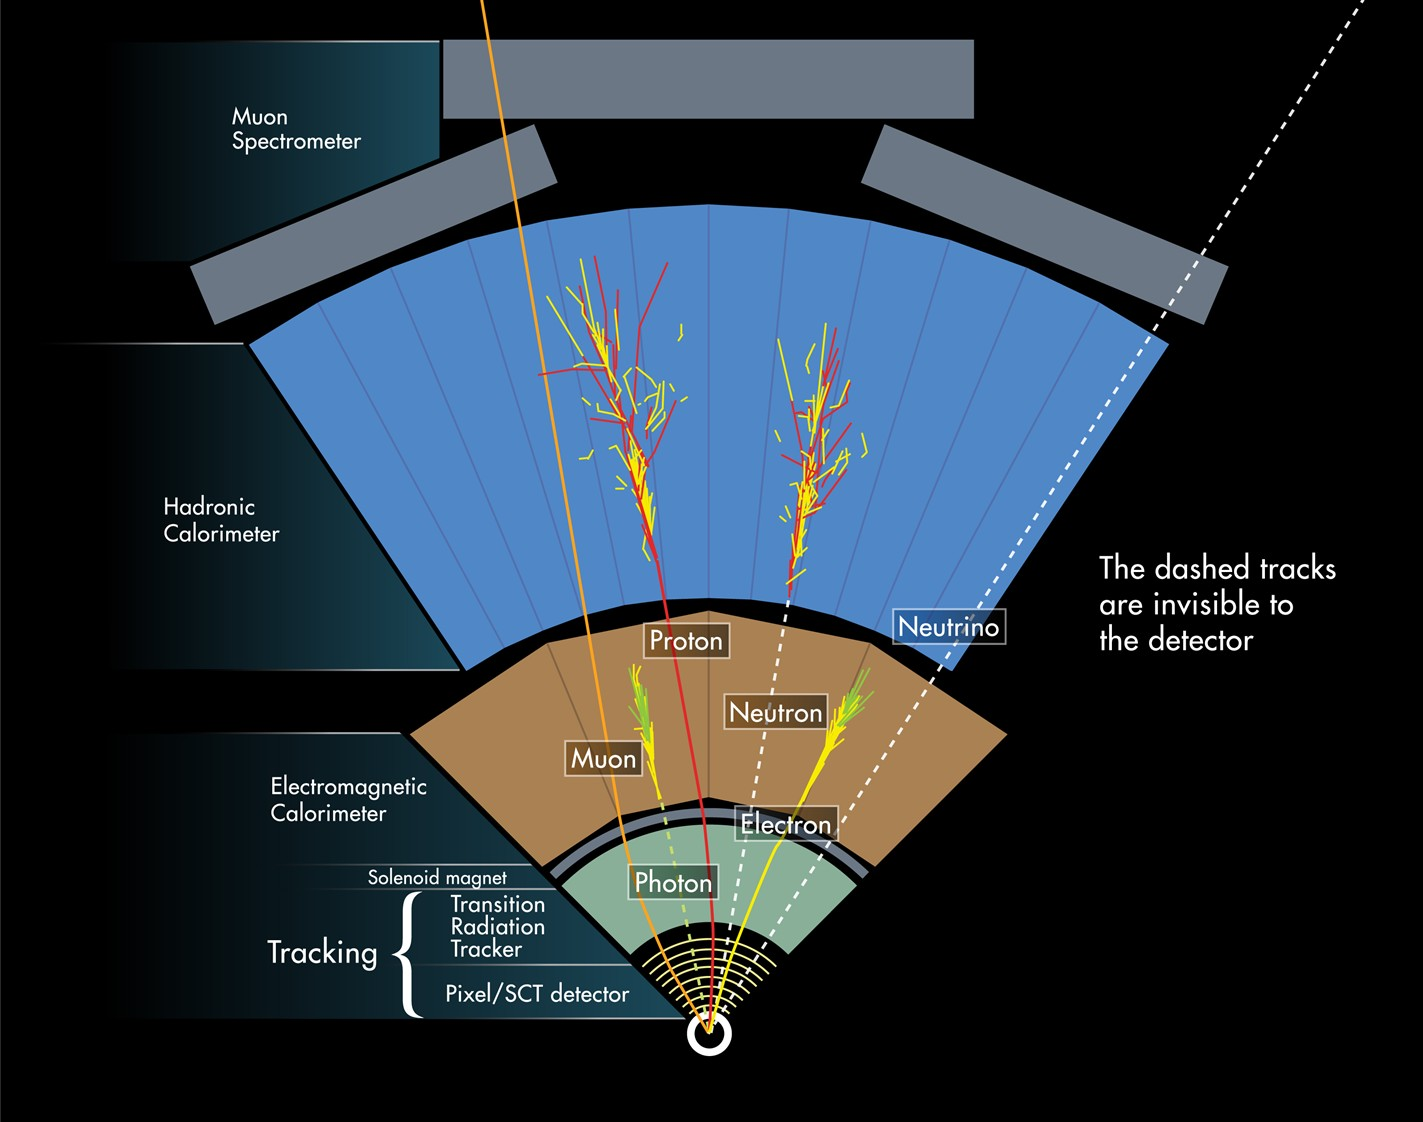
\includegraphics[width=0.80\textwidth,keepaspectratio]{figures/Reconstruction/ParticlePath}
\caption{
Schematics of the particle path
}
\label{fig:ParticlePath}
\end{center}
\end{figure}
\section{Tracks and Vertices}
The inner detector (ID) tracks are used for the reconstructions of the primary vertex and charged-particles kinematics.
The reconstruction of tracks~\cite{PERF-2015-08} starts with the formation of clusters of the hits in each ID component.
Three-dimentional space points are reconstructed from these clusters.
The track candidate is then selected with a set of space points by using combinatorial Kalman filter~\cite{FRUHWIRTH1987444}. 
The best track is selected using a scoring function, then finally the track is fitted and decided. 
The primary vertex, which represents the interaction point of the proton-proton collision, is reconstructed by fitting a common point to all reconstructed tracks~\cite{PERF-2015-01}. It is used to distinguish particles coming from the collision of interest from the ones produced by pileups.
\section{Calorimeter clusters} 
The topological cluster (topo-cluster) is used for reconstruction of each physics object. It is a four-momentum formed by cell signals of both the ECal and the HCal.
%The reconstruction of the hadron and jets is based on a three-dimensional topological clustering of individual calorimeter cell signals\cite{PERF-2014-07}.
The cluster is reconstructed following cell signal-significance patterns generated by electromagnetic and hadronic showers~\cite{PERF-2014-07}.
The clustering algorithm implicitly performs topological noise suppression by removing cells with insignificant signals which are not in close proximity to cells with significant signals. 
\section{Electrons}
%reconstruction
Electron candidates are reconstructed from topo-clusters in the ECAL matched to a track identified by the ID~\cite{ATL-PHYS-PUB-2017-022}.
\begin{figure}[tbp]
\begin{center}
 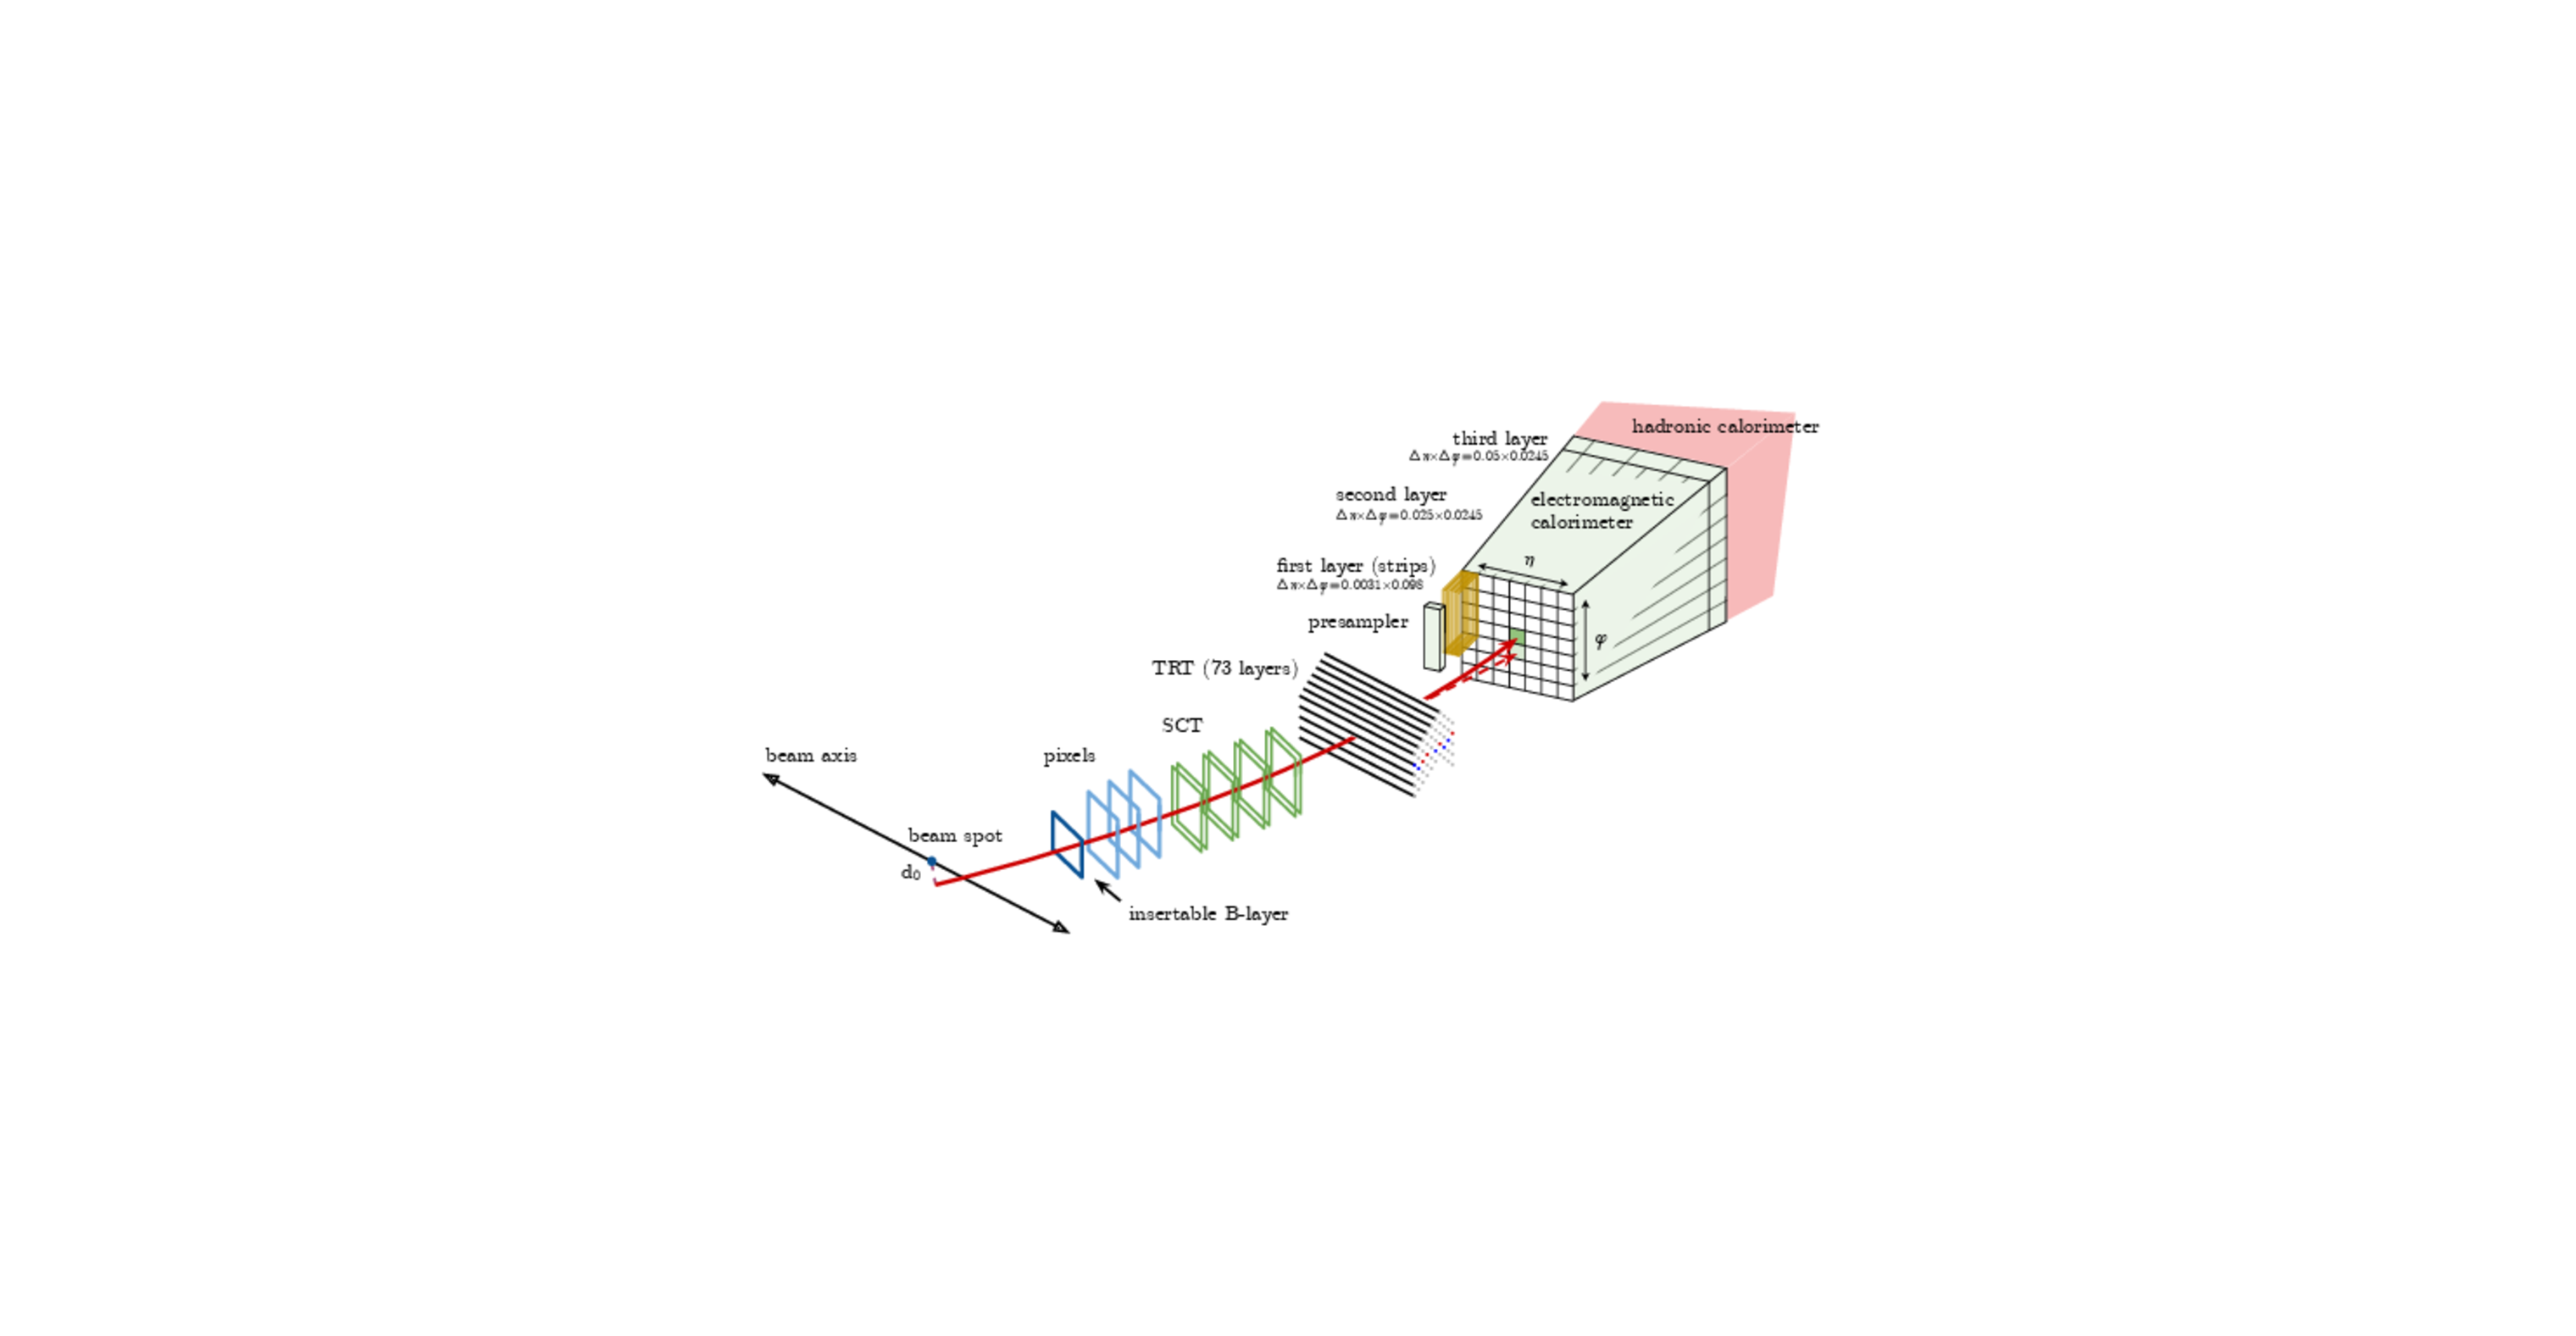
\includegraphics[width=0.80\textwidth,keepaspectratio]{figures/Reconstruction/electronPath}
\caption{
Schematics of the electron going through the detectors
}
\label{fig:electronPath}
\end{center}
\end{figure}
%identification
The reconstructed electron candidates are required to have $|\eta|<2.47$, excluding the transition region between barrel and endcap (1.37 < $|\eta|$ < 1.52).
A likelihood-based identification is required to reduce the backgrounds from photon conversion or hadrons, e.g. charged pion and $\pi^0 \rightarrow \gamma \gamma$. 
This identification algorithm combines various identification variables, like shower shape of the ECAL, the track conditions, and the matching of the tracks and the clusters. 
The ratio of the energy deposit in the HCAL to that of the whole ECAL cluster can be used to separate the electrons from the hadrons. 
The track requirement is useful to distinguish electrons from photons.
Electron candidates are categorized into three categories: LooseLH, MediumLH, and TightLH corresponding to 96\%, 94\%, 88\% of identification efficiencies to signal electrons at $E_\mathrm{T}$ = 100~GeV respectively, for the rejections of the backgrounds from misidentified hadrons, electrons from photon conversions, and non-isolated electrons originating from heavy-flavour decays. 
In this analysis, TightLH and LooseLH working points are employed.
%put calibration things here.....
The reconstruction and identification efficiencies are measured using  $J/\Psi \rightarrow ee$ and $Z\rightarrow ee$, $Z\rightarrow ee\gamma$ events~\cite{PERF-2017-01}. The efficiencies are shown in Figure~\ref{fig:recoElectron}. 
The discrepancy between the data and the MC is corrected by using event-weight scale factors, parametrized with $E_\mathrm{T}$ and $\eta$.
%put momentum? resolutions here
\begin{figure}[tbp]
\begin{center}
%\subfigure[]{
 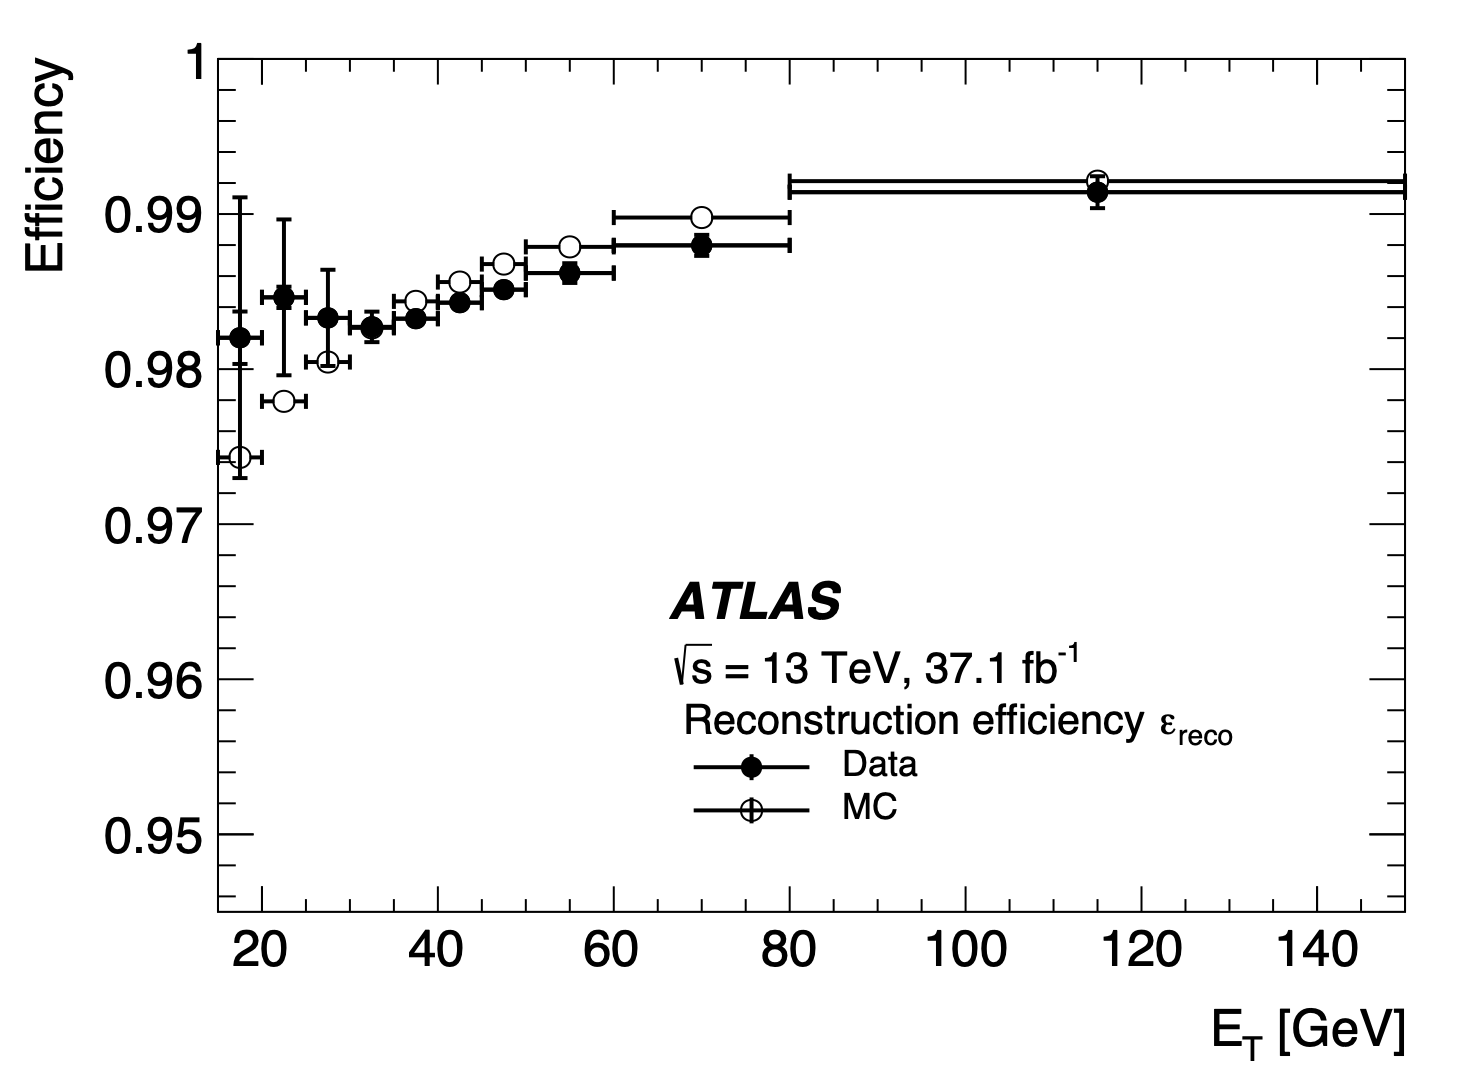
\includegraphics[width=0.50\textwidth,keepaspectratio]{figures/Reconstruction/recoElectron}
 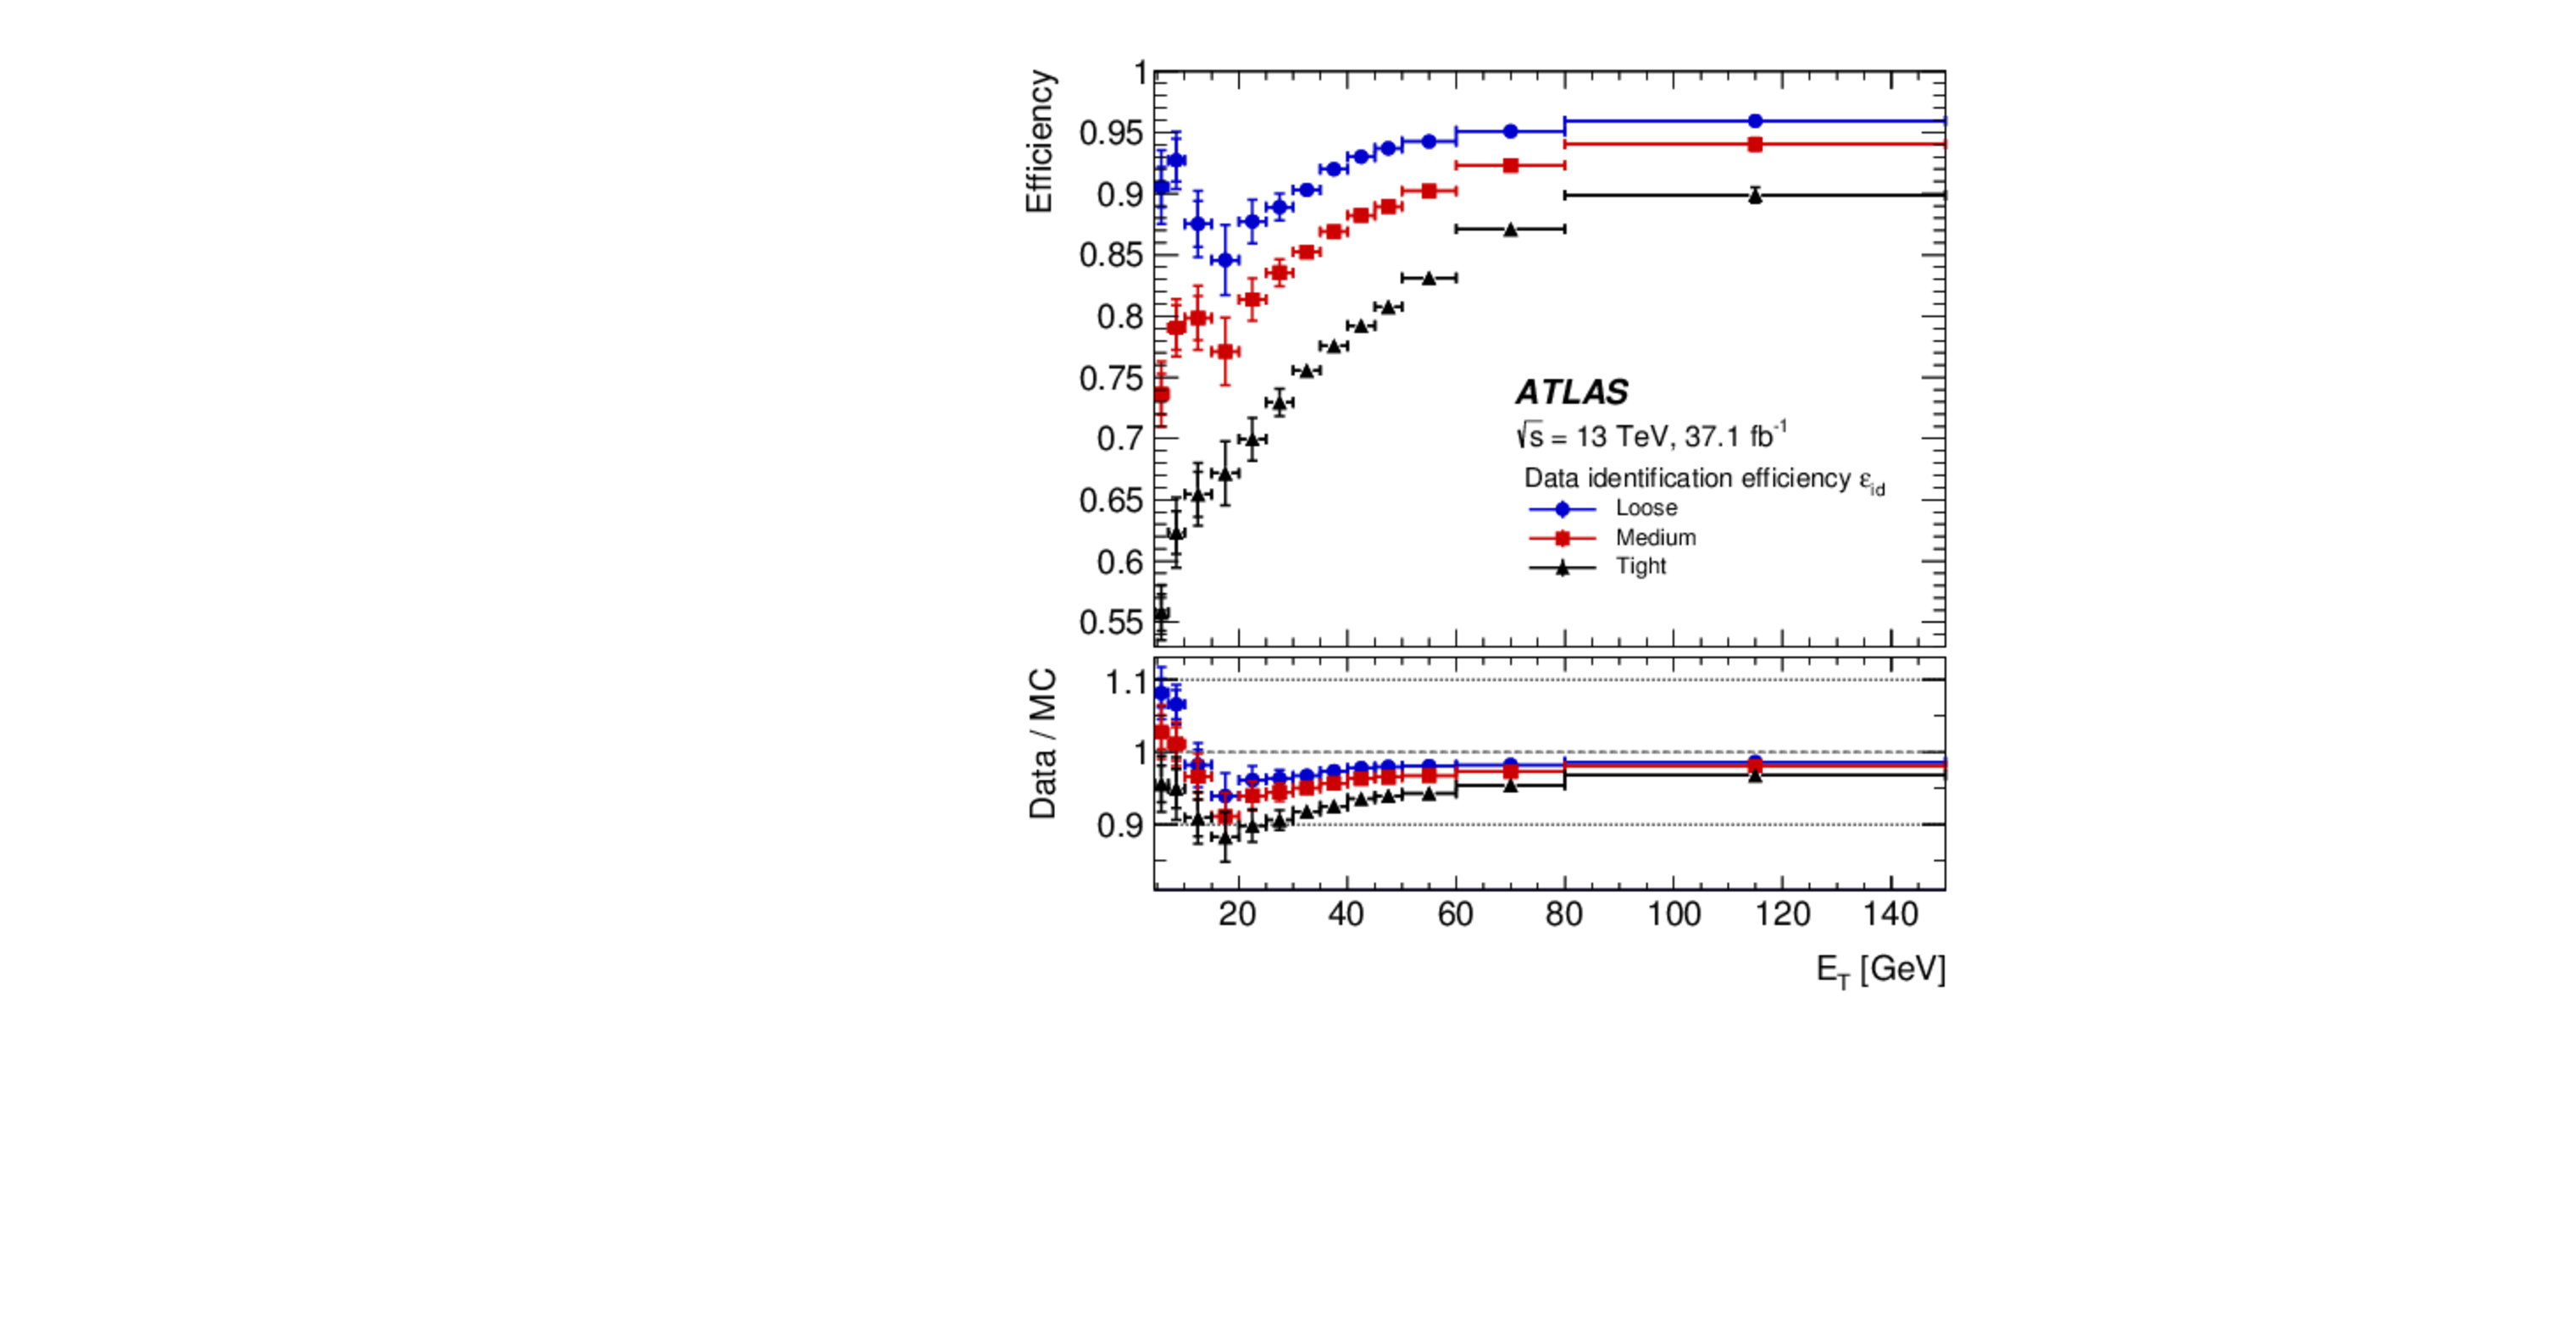
\includegraphics[width=0.45\textwidth,keepaspectratio]{figures/Reconstruction/idElectron}
%}
\caption{
electron reconstructing and identification efficiency with respect to the $E_\mathrm{T}$
}
\label{fig:recoElectron}
\end{center}
\end{figure}
Additional requirements are applied for isolation, to reduce the contamination of jets. 
The two isolation working points used in this analysis, which are determined by the track and ECAL information. 
The selections applied in this analysis are shown in the table~\ref{tab:electron_selection}.
Furthermore, track-to-vertex association requirements are applied. 
$d_0$ is the minimum distance between the primary vertex (PV) and the track, and $\sigma_{d_0}$ is its uncertainty. $z_0$ is the transverse impact parameter relative to the beamline.
\begin{table}[htbp]
\centering
\resizebox{0.8\textwidth}{!}{
\begin{tabular}[h]{|l|c|c|} \hline
                        & \emph{Loose}             & \emph{Tight}\\ \hline
  $p_\mathrm{T}$                 & 7~GeV                    & 30~GeV\\ \hline
  $|\eta|$              & \multicolumn{2}{c|}{$|\eta| < 2.47$ \notin [1.37,1.52]} \\ \hline
  Identification        & LooseLH                  & TightLH \\ \hline
  Isolation             & FCLoose $(p_\mathrm{T} <100~GeV)$ &  FixedCutHighPtCaloOnly \\
                        & no isolation requirement $( >100~GeV )$ & \\ \hline
$|d_{0}/\sigma_{d_0}|$  & \multicolumn{2}{c|}{ <~5 }\\  \hline
$| z_{0} \sin{\theta}|$ & \multicolumn{2}{c|}{ <~0.5~mm }\\ \hline
\end{tabular}
}
 \caption{Summary of electron selection used in this analysis}
 \label{tab:electron_selection}
\end{table}

\section{Muons}
%reconstruction
Muons are reconstructed by the combination of the tracks in the ID and Muon Spectrometer (MS)~\cite{PERF-2015-10}. 
%Figure~\ref{fig:recoMuon} shows the schematic diagram of the muon in the detectors.
%find and put the schematic of the muons
The reconstruction is performed by a simultaneous fit to the ID and MS information, taking also into account energy losses in the calorimeter.
%Several algorithms are used for the reconstruction: 
%combined (CB) muons which require independent tracks both in ID and the MS. CB muons are of highest quality, but have least acceptance. 
%Segment-tagged (ST) muons require an ID track with only one hit in the MS, which allows recovering the low-$p_T$ muons. 
%Calorimeter-tagged (CT) muons are reconstructed by requiring one ID track and energy deposits in the calorimeter, whose energy agrees with the expected value for a minimum-ionizing particle. 
%CT muons are used to increase the acceptance in the region of $|\eta| < 0.1$, corresponding to the region without the muon spectrometers due to the layout of the calorimeter cables. 
%identification
Muon identification is performed by applying quality requirements that suppress backgrounds, mainly from pion and kaon decays. 
Similarly to electrons, they are classified in three categories; Loose, Medium, and Tight which correspond to an efficiency of 98.1\%, 96.1\% and 91.8\% for muons with $p_\mathrm{T}$ = [20, 100]~GeV.
%It also selects prompt muons with high efficiency and/or guaranteeing a robust momentum measurement. 
%For Medium muons, the CB tracks required to have more than three hits in at least two MDT layers except for |$\eta$|<0.1.
%Specifically, the $q/p$ significance, defined as the absolute value of the difference between the ratio of the charge and momentum of the muons measured in the ID and MS divided by the sum in quadrature can be used for distinguish the muons.It is required to have less than seven for the contamination of the hadrons misidentified as muons.
%The Loose identification uses all types of Muons. 
%All CB and \textcolor{blue}{ME} muons satisfying the Medium requirements are included. 
The identification used in this analysis is shown in Table~\ref{tab:muon_selection}.
%reconstruction efficiency of calibration things
The muon reconstruction efficiencies are measured with samples of $J/\Psi \rightarrow \mu\mu$ and $Z\rightarrow \mu\mu$, as well as the momentum scale and resolution~\cite{MUON-2018-03}.
The reconstruction efficiency is found to be close to 99\% over most of the covered phase space ($|\eta|$ < 2.5 and 5 < $p_{T}$ < 100 GeV). 
The isolation efficiency varies between 93 and 100 \% depending on the selection applied and on the momentum of the muon. 
Both efficiencies are checked to be well reproduced in MC simulation. 
%In the central region of the detector, the momentum resolution is measured to be 1.7 \% (2.3 \%), and the momentum scale is known with an uncertainty of 0.05 \%. In the region $|\eta|$ > 2.2, the $p_T$ resolution for muons is 2.9 \% while the precision of the momentum scale for low-$p_T$ muons is about 0.2 \% \cite{}.
%The further instructions are shown in \cite{MUON-2018-03}.
%identification
\begin{table}[ht]
\centering
\resizebox{0.8\textwidth}{!}{
\begin{tabular}[ht]{|l|c|c|c|}
  \hline
  & \emph{Loose} & \emph{Tight}\\
  \hline
  \hline
  $p_\mathrm{T}$ & 7~GeV & 30~GeV\\
  \hline
  $|\eta|$ & \multicolumn{2}{c|}{$|\eta| < 2.5$} \\
  \hline
  Identification & Loose & Medium \\
  \hline
  Isolation &  FCLoose $(p_\mathrm{T} <100~GeV)$                   &  FixedCutHighPtCaloOnly \\
            &  no isolation requirement $( >100~GeV )$ & \\
  \hline
  $|d_{0}/\sigma_{d_0}|$ & \multicolumn{2}{c|}{ <~3 }\\ 
  \hline
  $| z_{0} \sin{\theta}|$ & \multicolumn{2}{c|}{ <~0.5~mm }\\
  \hline
 \end{tabular}}
 \caption{Summary of muon selection used in this analysis}
 \label{tab:muon_selection}
\end{table}
Similar to the electron, the isolation requirement is also applied to the muons, as shown in the Table~\ref{tab:muon_selection}.
\begin{figure}[tbp]
\begin{center}
%\subfigure[]{
 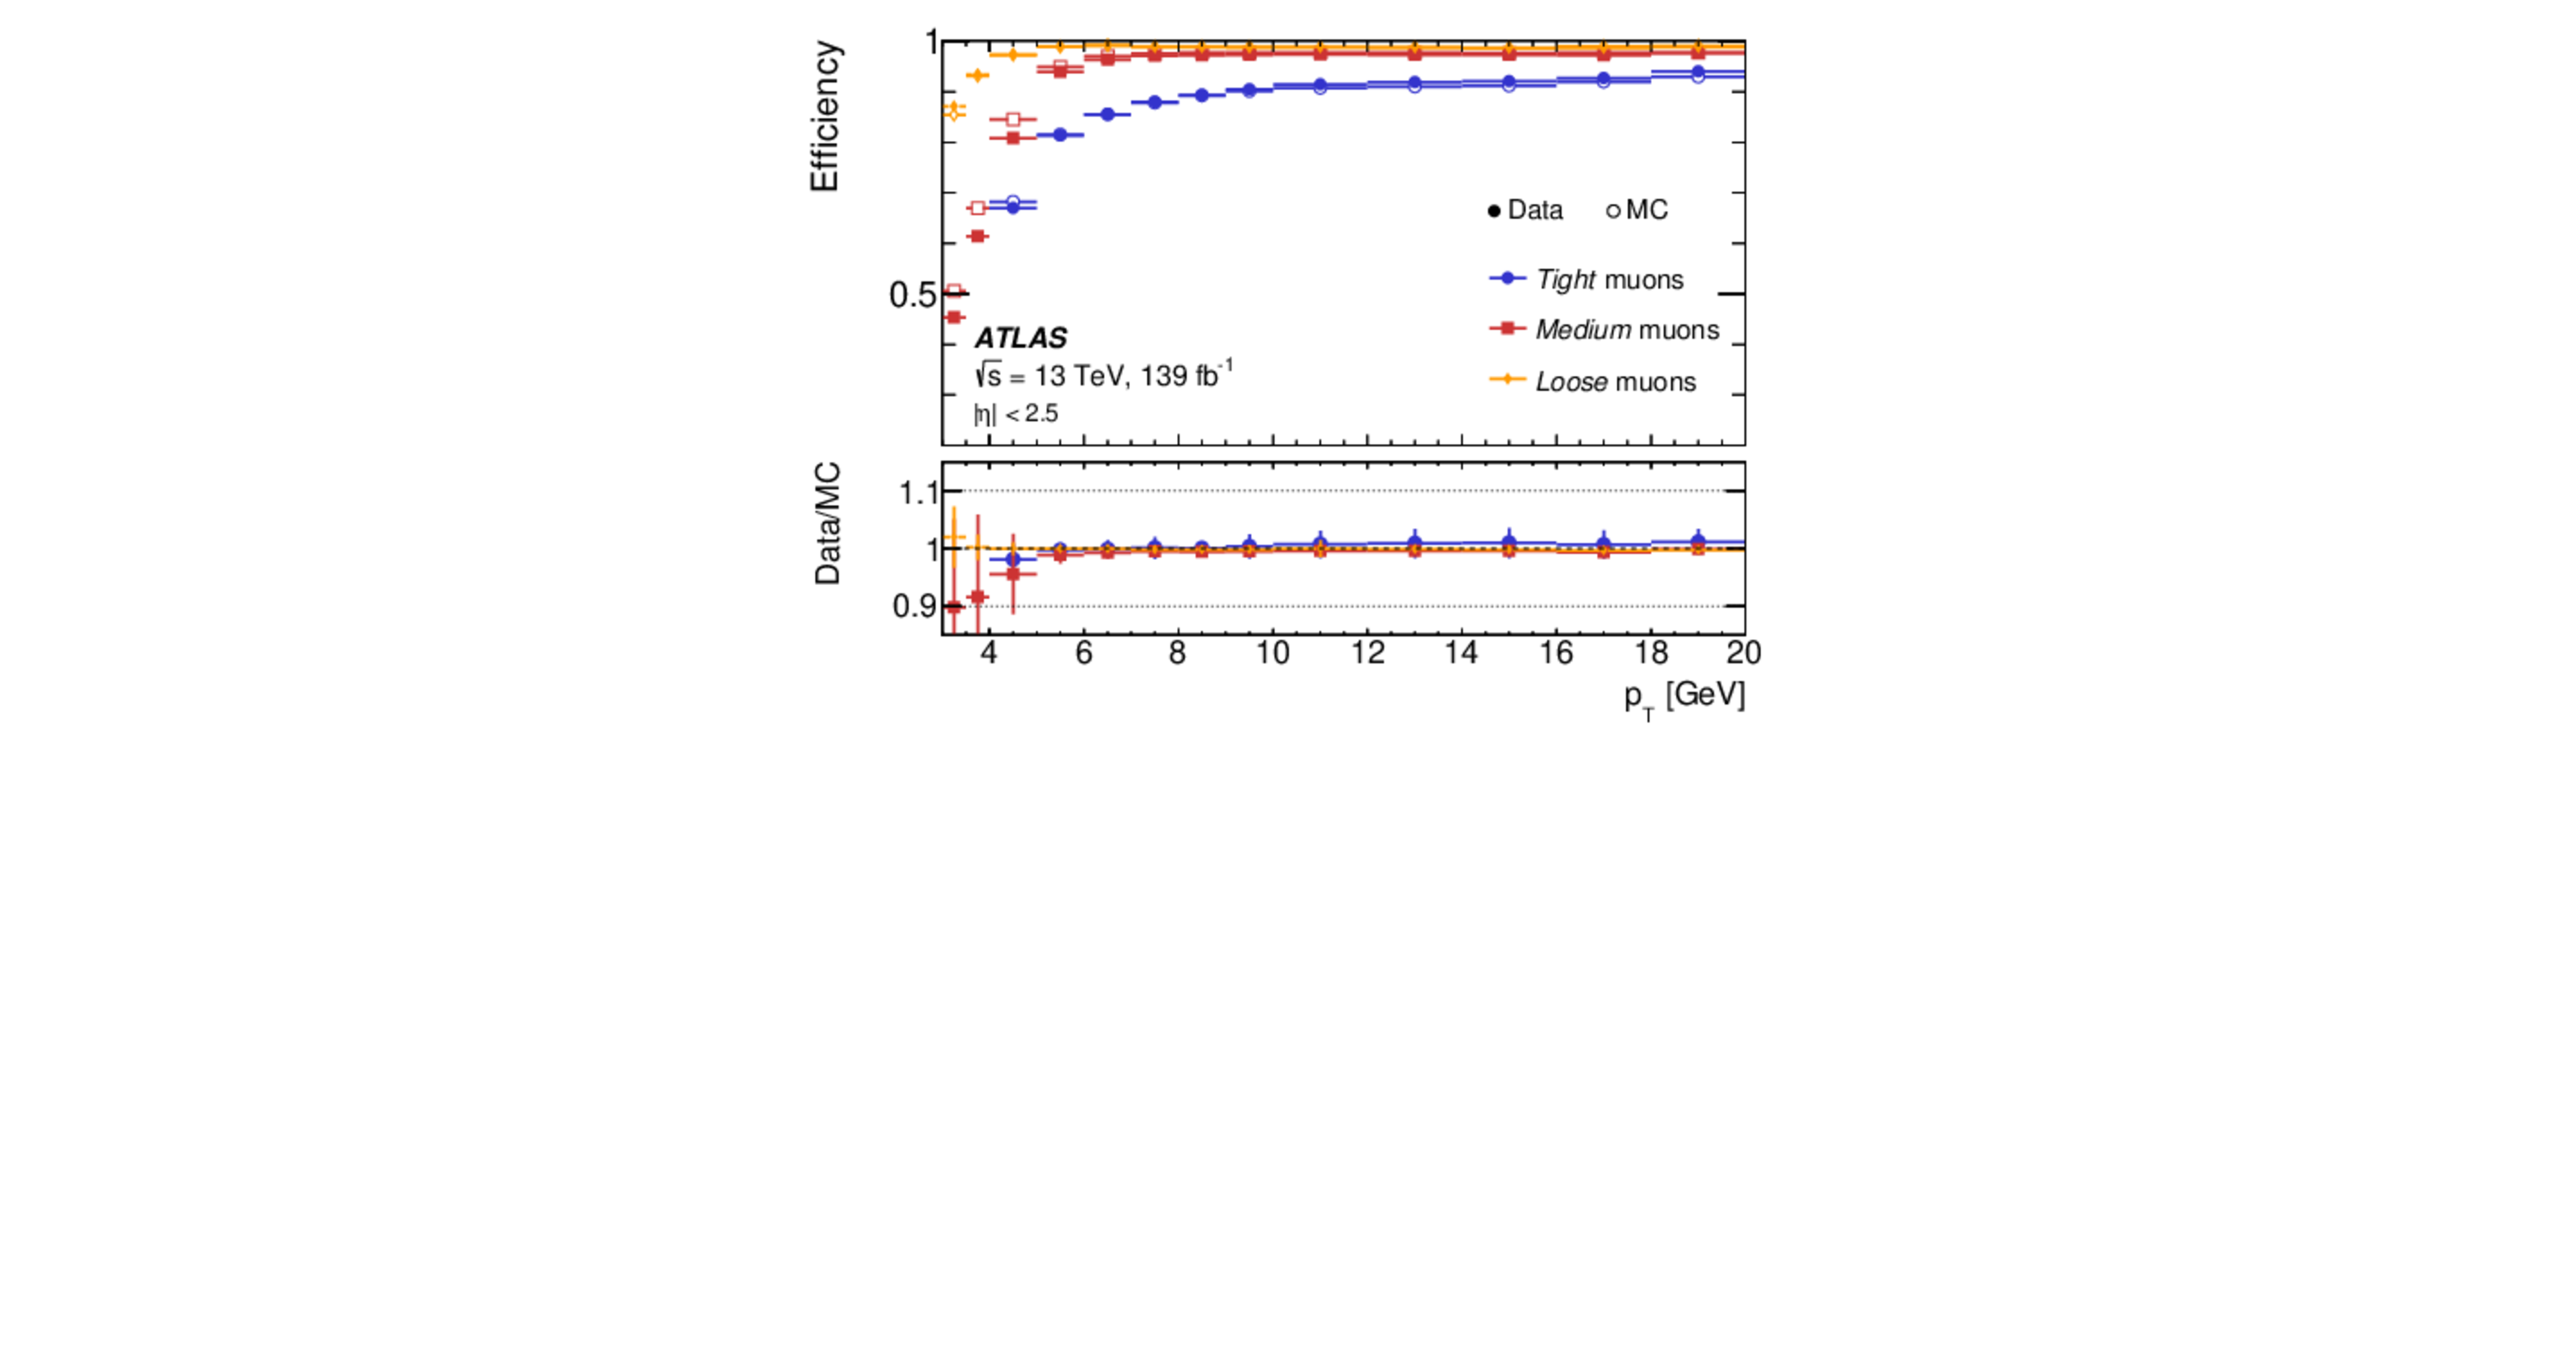
\includegraphics[width=0.45\textwidth,keepaspectratio]{figures/Reconstruction/recoMuonpT}
 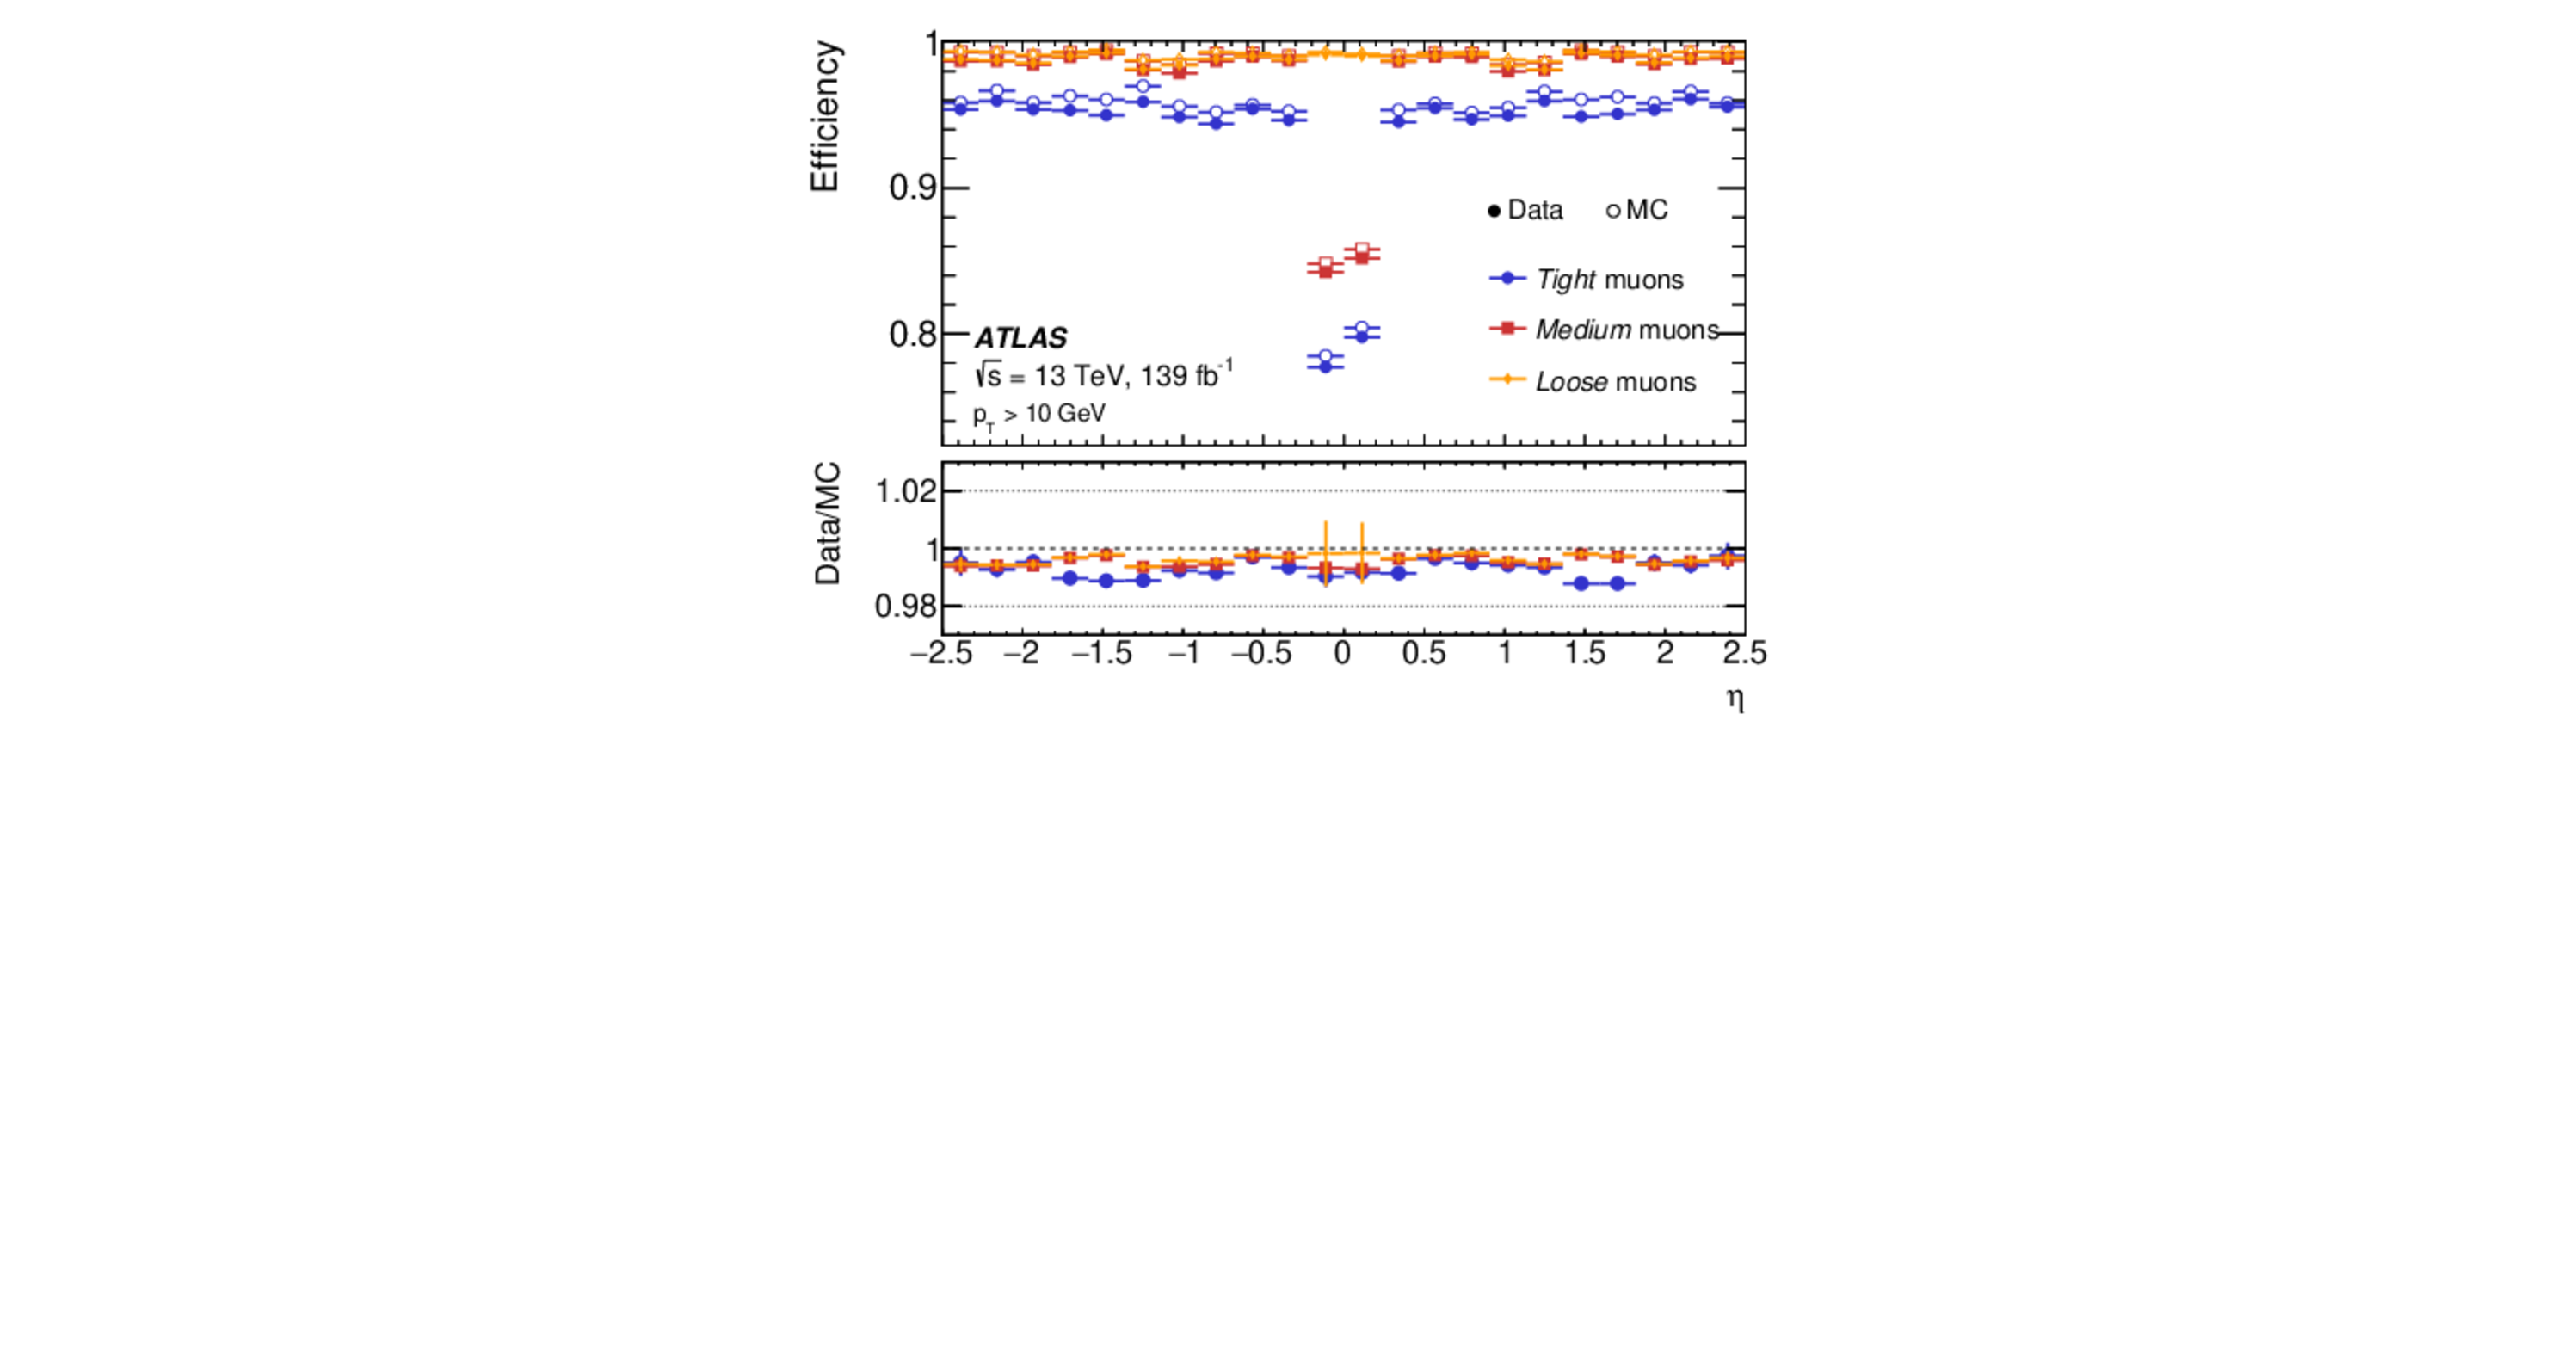
\includegraphics[width=0.45\textwidth,keepaspectratio]{figures/Reconstruction/recoMuonEta}
%}
\caption{
muon reconstructing and identification efficiency with respect to $p_\mathrm{T}$ (left) and $\eta$ (right) \cite{MUON-2018-03}
}
\label{fig:recoMuon}
\end{center}
\end{figure}
\section{Jets}
%Spray of hadrons produced by the hadronization of the final-state partons is called jets.
%Kinematics of jets ideally reflects the parton kinematics.
Jets are basically reconstructed by grouping topo-clusters by the anti-$k_t$ algorithm~\cite{Cacciari_2008}, with a radius of $R = 0.4$ (small-$R$ jets) or $R = 1.0$ (large-R jets). 
The small-R jet contains most of the radiation from the quark or gluon jets. 
The large-R jets represent the hadronic decays of the heavy, boosted objects where two jets from the quarks overlap.

The anti-$k_t$ algorithm defines a measure of distance $d_{ij}$ between the clusters in the calorimeter,
\begin{equation}
d_{i j}=\min \left\{\frac{1}{k_{\mathrm{T}, i}^{2}}, \frac{1}{k_{\mathrm{T}, j}^{2}}\right\} \times \frac{\left(\Delta R_{i j}\right)^{2}}{R^{2}}
\end{equation}
where $k_{T,i}$ is the transverse momentum of the cluster i and $\Delta R_{i j}=\sqrt{\left(\Delta y_{i j}\right)^{2}+\left(\Delta \phi_{i j}\right)^{2}}$ is the distance between the clusters $i$ and $j$ where $y$ is the rapidity. 
The algorithm searches for the minimum $d_{i j}(k)$ combinations and merges them. 
It iterates that procedure until $d_{i j}(k) = d_{i B}(k)$, where $d_{i B}(k) = \frac{1}{k^2_{ti}}$, where cluster i is regarded as a jet.
This procedure is repeated until all clusters are grouped into jets.
Figure~\ref{fig:antikt} shows how the clustering performed for example.
%?
%The small-R jets and the large-R jets are both reconstructed using topo-clusters, while only small-R jets use the track information to give better performance of measuring the energy and the momentum of the jets.
%?
\begin{figure}[tbp]
\begin{center}
%\subfigure[]{
 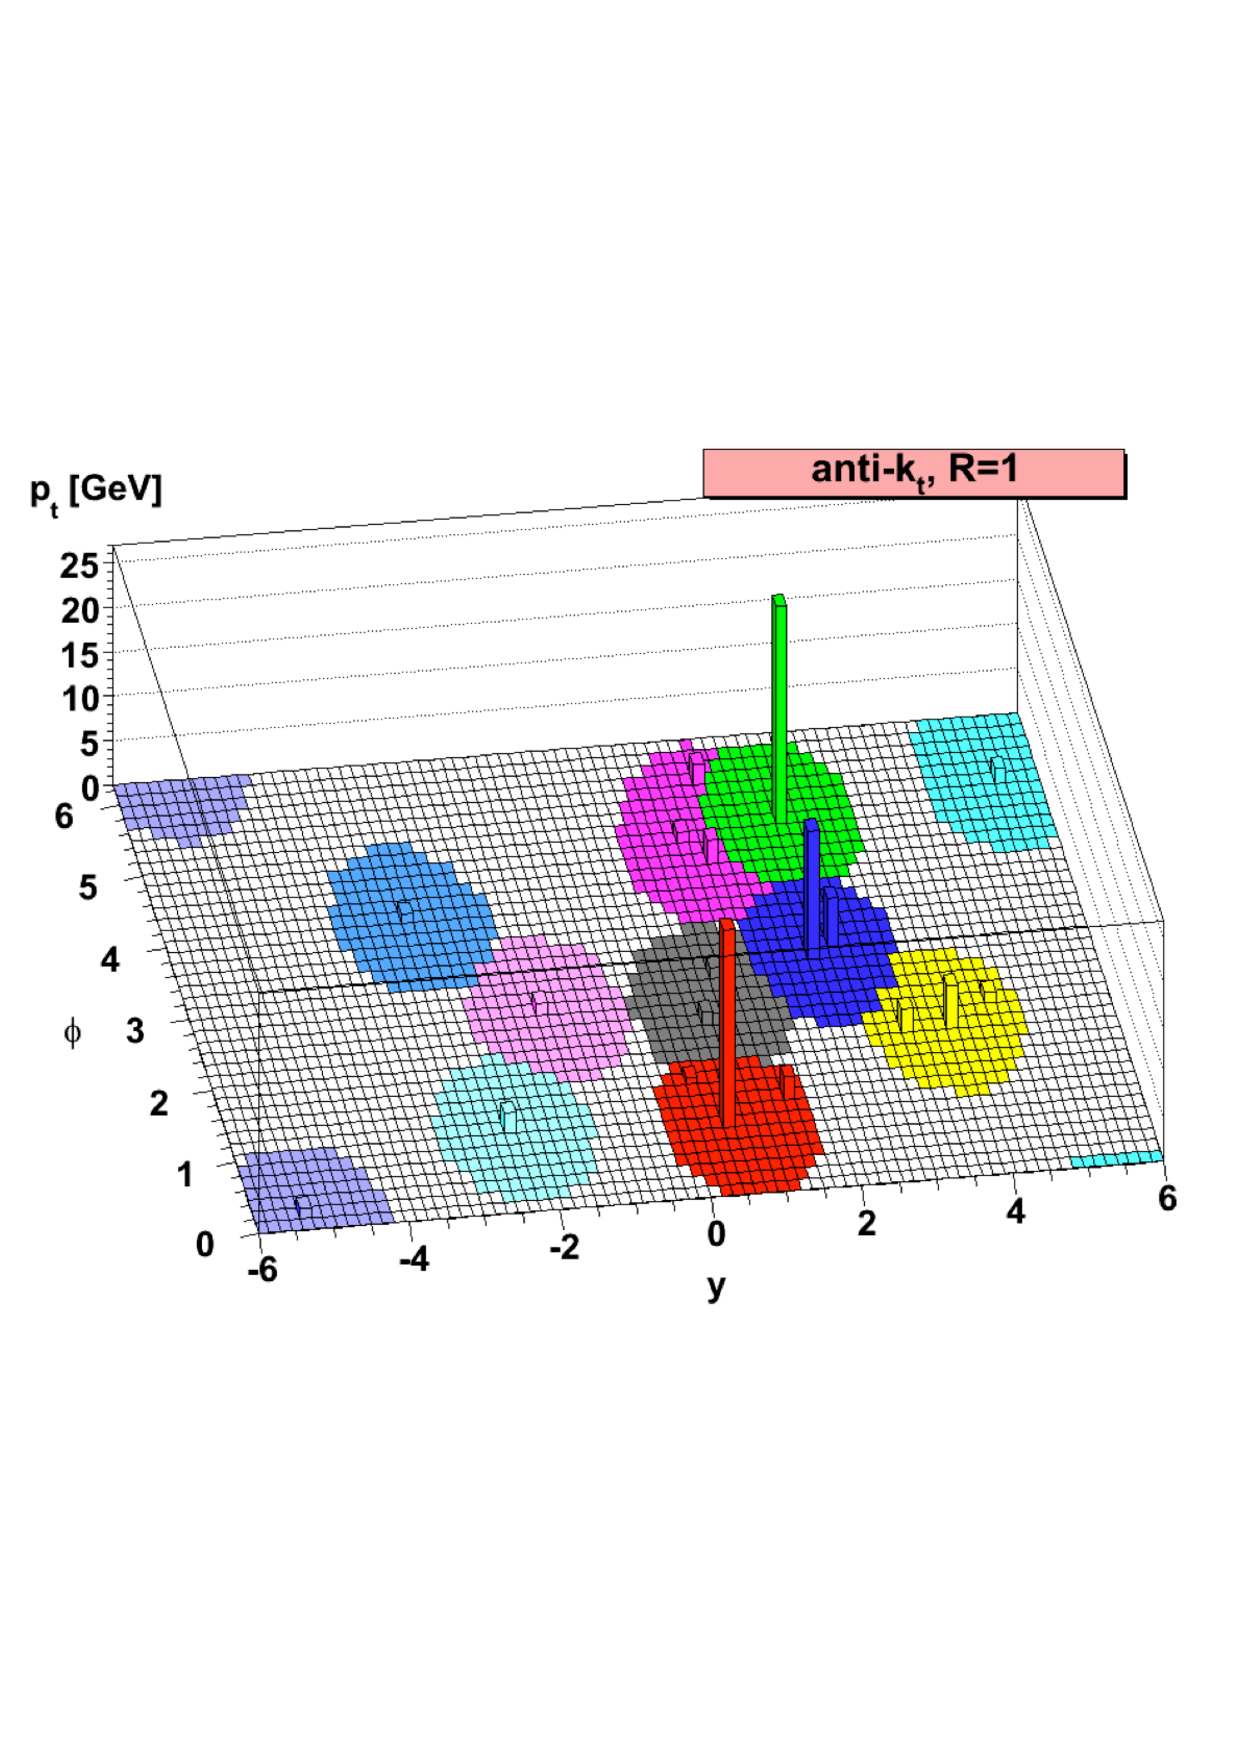
\includegraphics[width=0.60\textwidth,keepaspectratio]{figures/Reconstruction/antikt}
\caption{
anti-$k_T$ algorithm \cite{Cacciari_2008}
}
\label{fig:antikt}
\end{center}
\end{figure}

\subsection{Small-R Jets}
\label{subsec:sRjets}
The small-R jets are reconstructed using anti-$k_T$ algorithm with a radius of $R = 0.4$. The particle flow (PFlow) algorithm~\cite{PERF-2015-09} is used in order to prepare the inputs for the jet reconstruction.
The PFlow algorithm uses an ensemble of signals from the calorimeter and the ID to remove overlaps between the energy and the momentum measurements made in the calorimeter and the ID.
%PFlow algorithm
In the PFlow algorithm, firstly tracks from the ID are selected, then the tracks to corresponding topo-clusters are matched to them. 
The expected energy in the calorimeter, deposited by the particle that also created the track, is computed based on the topo-cluster position and the track momentum. For each track/topo-cluster system, the algorithm evaluates the probability that the particle energy was deposited in more than one topo-cluster. If this is found to be high, the algorithm adds more topo-clusters to the system, to recover the entire shower energy.
Finally, the expected energy deposited in the calorimeter by the particle is subtracted cell by cell from the topo-clusters assigned to the track.
If the energy left-overs in the calorimeter are found and if the remnants are compatible with the expected shower fluctuation of a single particle, they are removed. In the case they are significant, they are kept, assuming they were created by another neutral particle and are referred to as modified clusters. From the collection of tracks, those associated to the vertex of interest, as well as, modified or unmodified topo-clusters are used as inputs to the jet reconstruction.
The ID tracker information has better resolution for low-$p_\mathrm{T}$ particles, and better angular resolution and can trace the particles to hard-scatter
interaction or pile-up. On the other hand, calorimeters have better resolutions for high $p_\mathrm{T}$ and can get neutral particles. 
Therefore the combined information can improve energy and angular resolution, as well as reduce the pile-up contributions.

%calibration
The calibration for the PFlow jets are done with several steps in order to do the correction for all detector effects. 
\begin{itemize}
    \item \textbf{\sf{pileup-substruction}} \\
    The per-event pileup contributions to the $p_\mathrm{T}$ of each jet are removed based on each area. It is subtracted based residual $N_{PV}$ and $\mu$ (average interaction per crossing) \cite{JETM-2018-05}.
    The corrected jet $p_\mathrm{T}$ is described as:
    \begin{equation}
     p_{T}^{\text {corr }}=p_{T}^{\text {reco }}(-\rho \times A)-\alpha\left(N_{P V}-1\right)-\beta\langle\mu\rangle
    \end{equation}
    where $\rho$ is the median pile-up momentum density, $A$ is the jet area, respectively.
    This correction with repect to $\eta$ is shown in Figure~\ref{fig:pileup}.
    \begin{figure}[tbp]
    \begin{center}
    %\subfigure[]{
    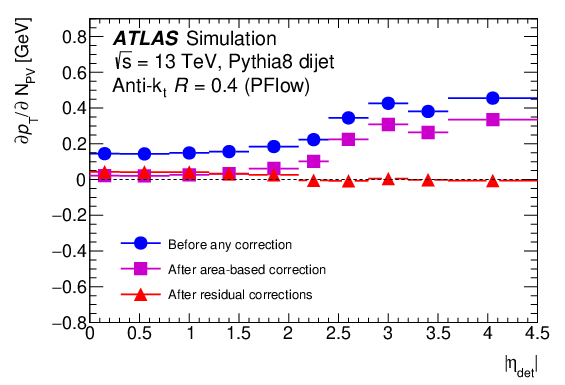
\includegraphics[width=0.45\textwidth,keepaspectratio]{figures/Reconstruction/intimepileup}
    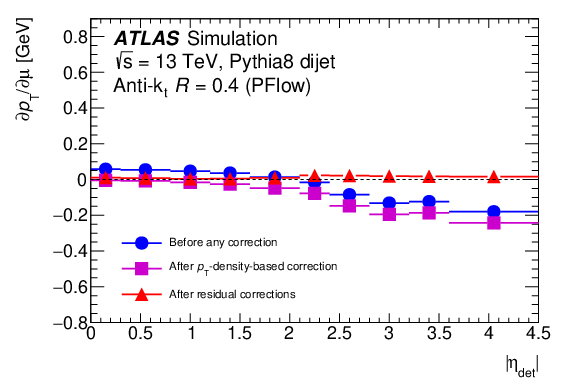
\includegraphics[width=0.45\textwidth,keepaspectratio]{figures/Reconstruction/outtimepileup}
    \caption{
    pile-up subtraction \cite{JETM-2018-05}
    }
    \label{fig:pileup}
    \end{center}
    \end{figure}
    \item \textbf{\sf{MC-based JES, $\eta$, calibration}} \\
    The ratio of the reconstructed jet $p_\mathrm{T}$ with the truth jet $p_\mathrm{T}$ strongly depends on the detector position. 
    Truth jets are built from stable particles in the MC generator event record. 
    Some corrections are applied as a function of E and $\eta$, by comparing the reconstructed jets to truth jets (energy response, $\mathrm{E}^{\text {reco }} / \mathrm{E}^{\text {truth }}$ )~\cite{JETM-2018-05}.
    Figure~\ref{fig:JES} shows the jet energy response as a function of $\eta$.
    \begin{figure}[tbp]
    \begin{center}
    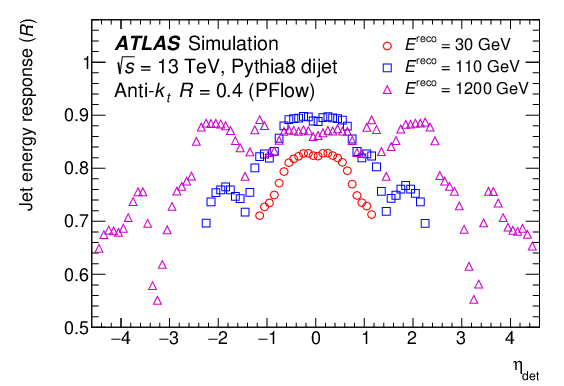
\includegraphics[width=0.50\textwidth,keepaspectratio]{figures/Reconstruction/JES}
    \caption{
    Jet energy response \cite{JETM-2018-05}
    }
    \label{fig:JES}
    \end{center}
    \end{figure}
    \item \textbf{\sf{Global sequential calibration}} \\ 
    The Global Sequential Calibration (GSC) is applied, mainly to account for the different responses to quark and gluon-initiated jets. 
    This calibration procedure reduces flavour dependence and energy leakage effects using calorimeter, track, and muon-segment variables.
    It also includes the correction for the punch-through, which happens for jets with large $p_\mathrm{T}$ whose energy is not fully contained in calorimeter \cite{JETM-2018-05}. The dependence of the n$_{\mathrm{trk}}$ on $p_\mathrm{T}$ response is shown in figure~\ref{fig:GSC}.
    \begin{figure}[tbp]
    \begin{center}
    %\subfigure[]{
    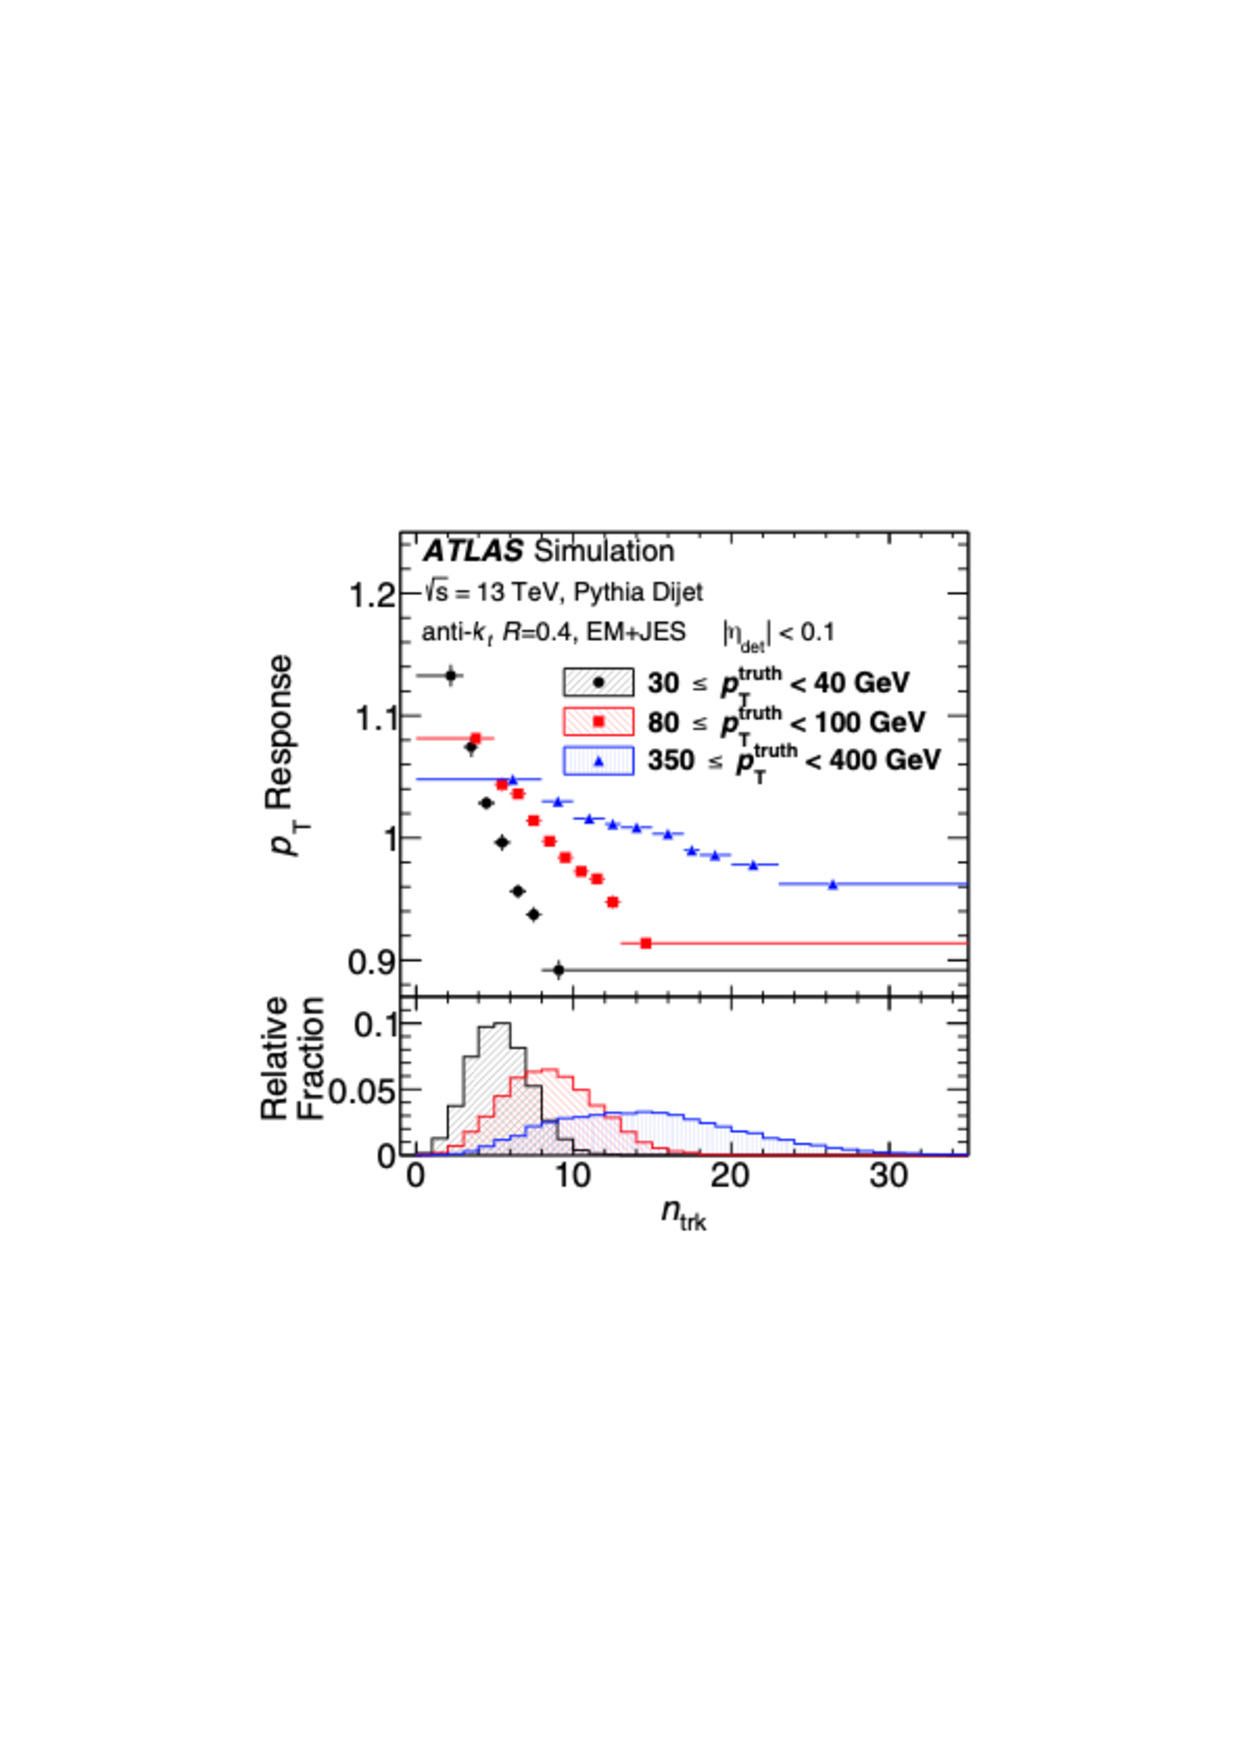
\includegraphics[width=0.4\textwidth,keepaspectratio]{figures/Reconstruction/GSC2}
    \caption{
      \cite{JETM-2018-05}
    }
    \label{fig:GSC}
    \end{center}
    \end{figure}
    \item \textbf{\sf{In-situ calibration}} \\
    The last calibration step is a correction with respect to the data. 
    This is an adjustment for the potential differences between data and MC, and this is only applied to the data.
    %This calibration uses methods that rely on well-calibrated reference objects in the event to constrain the jet $p_T$ response. 
    The jet response is estimated by balancing the jet $p_\mathrm{T}$ to a well-measured recoil object. 
    %There are three stages of in situ measurements. 
    The first procedure denotes intercalibration, corrects the JES of forward jets to agree with that of central jets, by exploiting the $p_\mathrm{T}$ balance in dijet events. 
    In the second procedure corrections are derived by balancing the jet $p_\mathrm{T}$ against a calibrated Z boson or photon (Z+jet and $\gamma$+jet analyses). 
    Finally in the procedure called the multijet balance, a system of well-calibrated low $p_\mathrm{T}$ jets is used to calibrate a single high $p_\mathrm{T}$ jet. %The second and third stages are usually estimated only for central jets. However, thanks to the eta-intercalibration stage the corrections are applicable to forward jets as well. 
    Sets of the measurements are combined to give a continuous calibration curves of the ratio of the jet response as a function of jet $p_\mathrm{T}$, shown in Figure~\ref{fig:in-situcalibration}.
    The jet energy resolution (JER) is also measured in-situ. 
    The JER is usually derived in dijet events by exploiting momentum conservation.
    \begin{figure}[tbp]
    \begin{center}
    %\subfigure[]{
    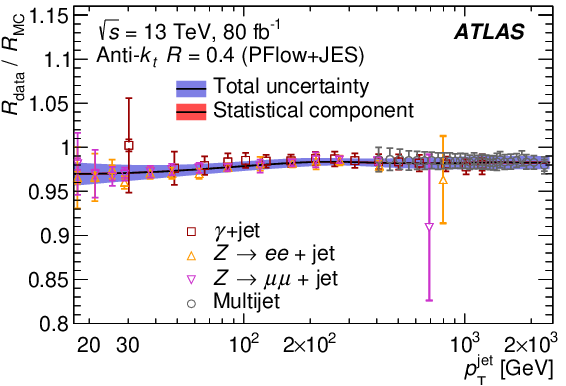
\includegraphics[width=0.5\textwidth,keepaspectratio]{figures/Reconstruction/insitucalibration}
    \caption{
    in-situ calibration \cite{JETM-2018-05}
    }
    \label{fig:in-situcalibration}
    \end{center}
    \end{figure}
\end{itemize}
%The total jet energy scale uncertainty with respect to these calibration is shown in Figure~\ref{fig:allJES}.
\begin{figure}[tbp]
    \begin{center}
    %\subfigure[]{
    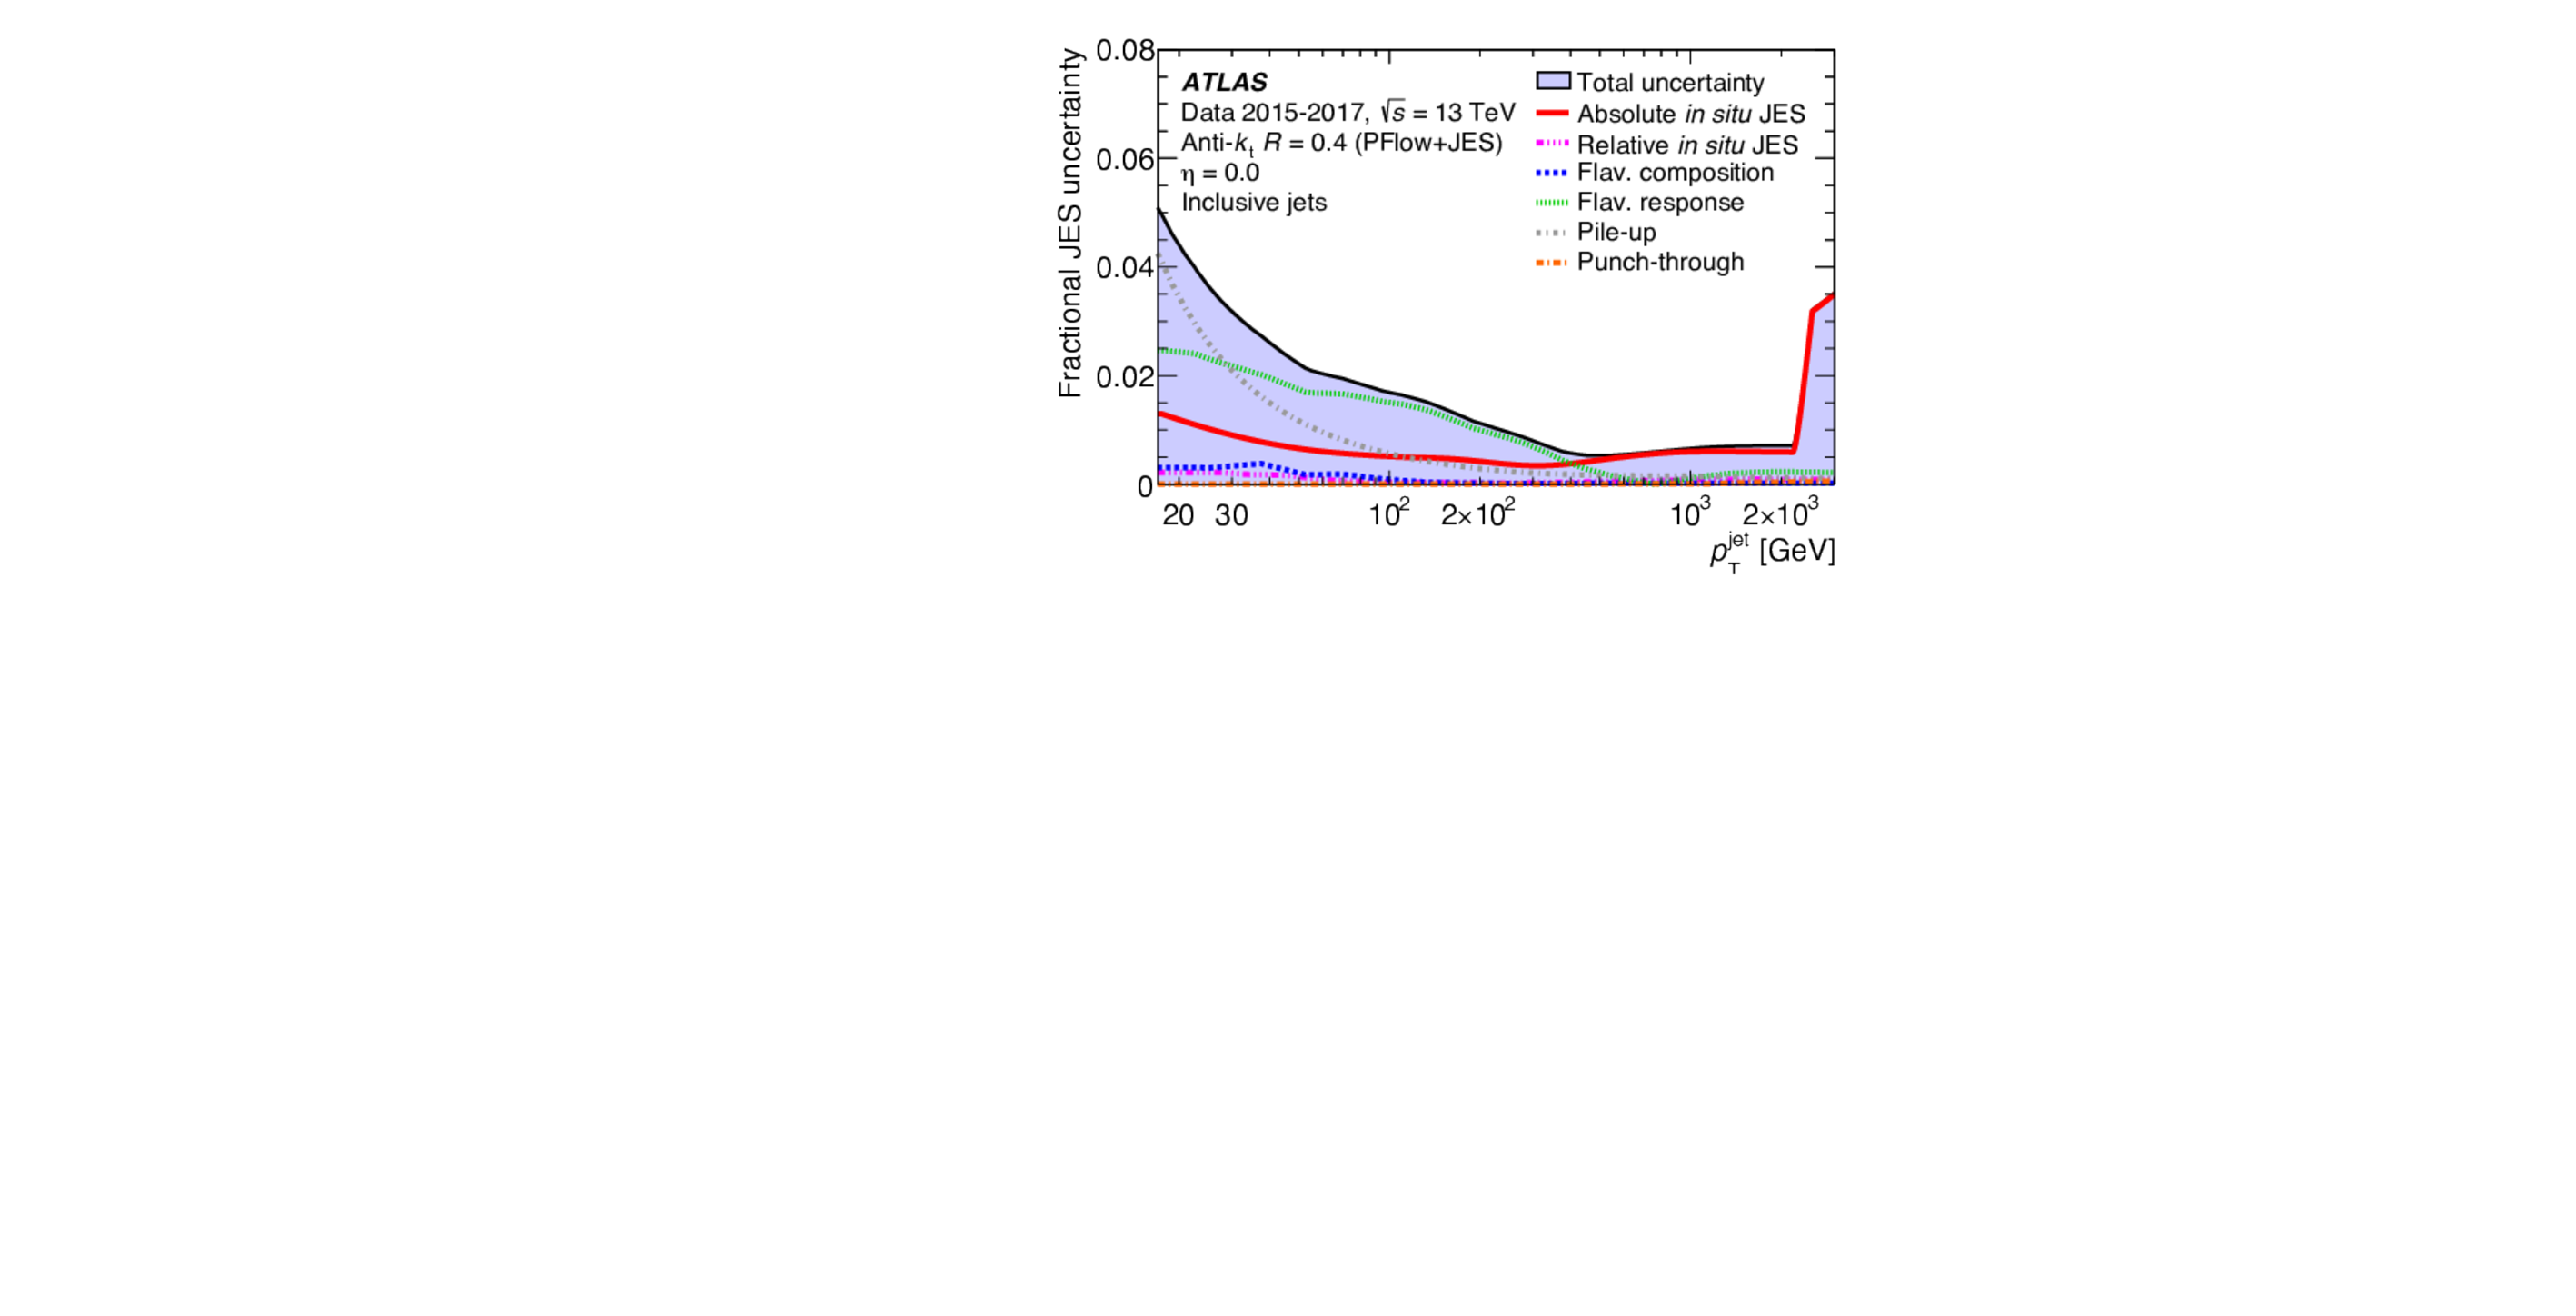
\includegraphics[width=0.5\textwidth,keepaspectratio]{figures/Reconstruction/allJES}
    \caption{
    All JES-related uncertainties is shown in black line. \cite{JETM-2018-05}
    }
    \label{fig:in-situcalibration}
    \end{center}
\end{figure}
%identification
The jet vertex tagger (JVT) is applied to identify the jets only from the hard interaction. 
Furthermore, in the context of the pile-up suppression, forward jet vertex tagger (fJVT) has been introduced, motivated by the forward-like topology in this analysis.
The b-tagging is used for rejecting the jets tagging including the b-hadrons, to suppress the top contributions.
\subsubsection{Jet Vertex Tagger}
The Jet Vertex Tagger (JVT)~\cite{PERF-2014-03} is constructed using a two-dimensional likelihood derived from the combination of two jet variables, corrJVF and $R^0_{p_\mathrm{T}}$;
\begin{equation}
\text { corrJVF }=\frac{\sum p_{\mathrm{T}}^{\text {track }}\left(\mathrm{PV}_0\right)}{\sum p_{\mathrm{T}}^{\text {track }}\left(\mathrm{PV}_0\right)+\frac{\sum_{i \geq 1} \sum p_{\mathrm{T}}^{\text {track }}\left(\mathrm{PV}_i\right)}{k \cdot n_{\mathrm{trk}}^{\mathrm{PU}}}}
\end{equation}
and
\begin{equation}
R_{p_{\mathrm{T}}}^0=\sum_{\text {trk }} \frac{p_{\mathrm{T}}^{\mathrm{trk}}\left(\mathrm{PV}_0\right)}{p_{\mathrm{T}}^{\text {jet }}}
\end{equation}
where PV$_i$ is the reconstructed vertex $i$ of the event. $i$ = 0 represents the primary vertex. The $\sum p_{\mathrm{T}}^{\text {track }}\left(\mathrm{PV}_0\right)$ is the scalar sum of the $p_\mathrm{T}$ of the tracks that are associated with the jet and originate from the primary vertex (PV$_0$), and $\sum_{i \geq 1} \sum p_{\mathrm{T}}^{\text {track }}\left(\mathrm{PV}_i\right)$ represents the scalar $p_\mathrm{T}$ sum of the tracks that are associated with the jet and originate from pile-up vertices. $k$ is a constant ($k$ = 0.01), in order to suppress the pileup dependence, and $n_{\text {trk }}^{\mathrm{PU}}$ denotes the total number of pileup tracks in an event. The distributions of two variables are shown in figure~\ref{fig:JVT}. 
%In the final JVT discriminant, jets with JVT values close to one are accepted as most likely being from primary vertex, while smaller JVT value are tagged as pile-up jets.
\begin{figure}[tbp]
    \begin{center}
    %\subfigure[]{
    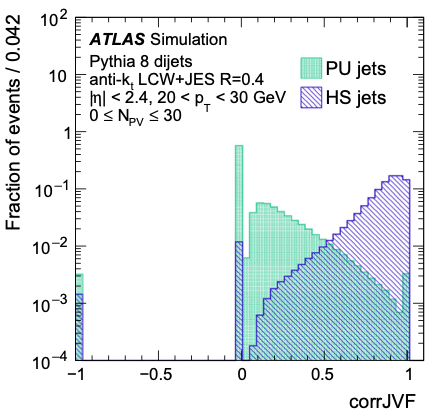
\includegraphics[width=0.34\textwidth,keepaspectratio]{figures/Reconstruction/corrJVF}
    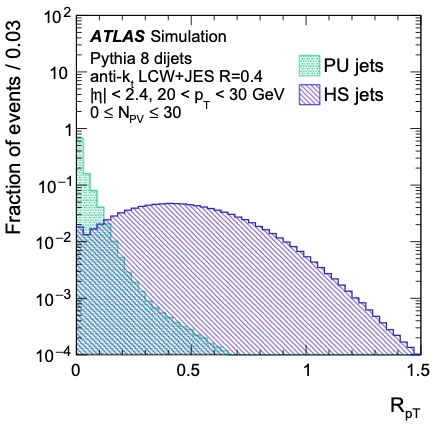
\includegraphics[width=0.32\textwidth,keepaspectratio]{figures/Reconstruction/RPT}
    \caption{
    Distributions of corrJVF (left) and R$_{p_{T}}$ (right) for PileUp jets and Hard Scattering jets. \cite{PERF-2014-03}
    }
    \label{fig:JVT}
    \end{center}
\end{figure}
\subsubsection{forward Jet Vertex Tagger}
The forward jet vertex tagger (fJVT)~\cite{PERF-2016-06} employs momentum conservation in order to tag a forward PFlow jet.
First central jets (jets with $|\eta|$ < 2.5.) are reconstructed per every vertex, and the relevant calibration is applied. 
The QCD pile-up jets are identified by using JVT and the $R^i_{p_\mathrm{T}}$ discriminant:
\begin{equation}
R_{p_{\mathrm{T}}}^i=\sum_{\mathrm{trk}} \frac{p_{\mathrm{T}}^{\mathrm{trk}}\left(\mathrm{PV}_i\right)}{p_{\mathrm{T}}^{\mathrm{jet}}}
\end{equation}
defined as the scalar $p_\mathrm{T}$ sum of the tracks that are associated with the jet and originate from the pile-up vertex $i$ divided by the fully calibrated jet $p_\mathrm{T}$. 
The missing transverse momentum per vertex $i$ ($p^{miss}_{\mathrm{T},i}$) is then calculated as
\begin{equation}
\mathbf{p}_{\mathrm{T}, i}^{\text {miss }}=-\left(\sum_{\text{jets,}{~p_{\mathrm{T}}^{\text{jet}}>20\mathrm{GeV}}} \mathbf{p}_{\mathrm{T}}^{\text {jet }}+\sum_{\text {tracks},~p_{\mathrm{T}}^{\text {jet }}<20 \mathrm{GeV}} \mathbf{p}_{\mathrm{T}}^{\text {track }}+\sum_{\text {tracks, jets fail } R_{p_{\mathrm{T}}}^i \text { cut }} \mathbf{p}_{\mathrm{T}}^{\text {track }}\right)
\end{equation}
For every forward jet fj, (jet in 2.5 < $|\eta|$ < 4.5.), the normalized projection of $p^{miss}_{\mathrm{T},i}$ on the direction of the forward jet,
\begin{equation}
\mathrm{fJVT}_i=\frac{\mathbf{p}_{\mathrm{T}, i}^{\text {miss }} \cdot \mathbf{p}_{\mathrm{T}}^{\mathrm{fj}}}{\left|\mathbf{p}_{\mathrm{T}}^{\mathrm{fj}}\right|^2}
\end{equation}
is computed. The final forward JVT (fJVT) discriminant is defined as
\begin{equation}
\mathrm{fJVT}=\max \left(\mathrm{fJVT}_i\right)
\end{equation}
The distributions of fJVT variable is shown in figure~\ref{fig:fJVT}. 
\begin{figure}[tbp]
    \begin{center}
    %\subfigure[]{
    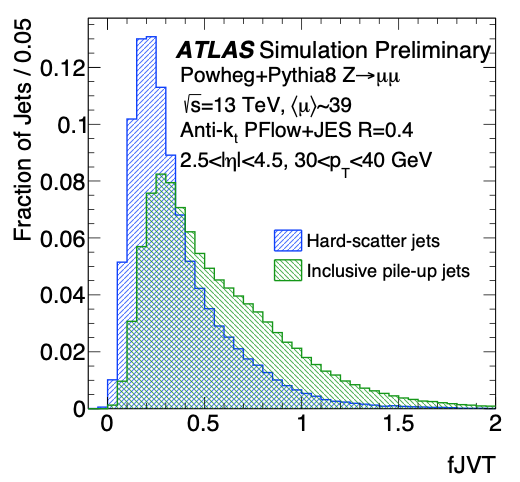
\includegraphics[width=0.34\textwidth,keepaspectratio]{figures/Reconstruction/fJVT}
    \caption{
    Distributions of fJVF for PileUp jets and Hard Scattering forward jets in 30<$p_\mathrm{T}$<40~GeV. \cite{PERF-2016-06}
    }
    \label{fig:fJVT}
    \end{center}
\end{figure}
\subsubsection{B-tagging}
The small-R jets containing a b-hadron are called b-jets and identified by performing b-tagging.
The algorithm makes use of the characteristics of the b-hadron whose lifetime is long enough to travel several mm from the primary interaction point before decaying, and create secondary vertices. These can be reconstructed using the tracks from the inner detector.
Additional kinematic properties of b-jets such as the mass and the momentum are also used in order to enhance separation with c-jets or light-jets originating from u-, d-, s- quarks or gluons.
The DL1r algorithm~\cite{ATL-PHYS-PUB-2020-009}, using a deep-learning neural network, is adopted in this analysis.
%The DL1r b-tagging is based on the features of b-hadrons in terms of the impact parameter of tracks and the displaced vertices reconstructed in the inner detector.
The DL1r combines four low-level taggers, IP3D~\cite{ATL-PHYS-PUB-2017-013}, SV1~\cite{ATL-PHYS-PUB-2017-011}, JetFitter~\cite{ATL-PHYS-PUB-2018-025}, and RNNIP~\cite{ATL-PHYS-PUB-2017-003}.
The IP3D uses signed impact parameter significance. The impact parameter, $d_0$ denotes the distance between tracks and the primary vertex.
%as shown in Figure~\ref{fig:bdecay}.
The SV1 reconstructs the secondary vertex in a jet. The JetFitter reconstructs the topology of b/c-hadron decay chains using Kalman filter~\cite{FRUHWIRTH1987444}.
Additionally, the RNNIP uses the track features including the track quality information.
Finally the DL1r combines the outcomes all of these four low-level taggers by deep-learning neural network algorithm.
Figure~\ref{fig:btageff} shows the efficiency of b-tagging with respect to jet $p_\mathrm{T}$.
In this analysis the b-tagging working point is fixed at 70\% efficiency.
\begin{figure}[tbp]
    \begin{center}
    %\subfigure[]{
    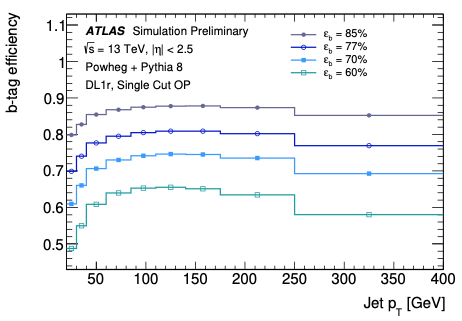
\includegraphics[width=0.50\textwidth,keepaspectratio]{figures/Reconstruction/btageff}
    \caption{
    Distributions of fJVF (left) for PileUp jets and Hard Scattering forward jets in 30<$p_\mathrm{T}$<40~GeV. \cite{ATL-PHYS-PUB-2020-009}
    }
    \label{fig:btageff}
    \end{center}
\end{figure}
\subsection{Large-R Jets}
The hadronic decaying objects from high-$p_\mathrm{T}$ W/Z boson cannot be separated as two small-R jets with large Lorentz boosts~\cite{JETM-2018-06} and the angle between quarks is small, hence they are reconstructed as one large-R jet.
Large-R jets are reconstructed with topo-cluster using anti-$k_T$ algorithm with R = 1.0. 
The calibration applied for the large-R jets is mainly the same as the procedure with the small-R jets, described in subsection~\ref{subsec:sRjets}, though there are some specific calibrations for large-R jets.
What is specific to the large-R jet is that the reconstructed topo-clusters are highly contaminated by the calorimeter noises, particles from pile-up, soft radiations. Therefore it is first applied grooming and then applied MC and in-situ calibrations. 
\begin{itemize}
    \item \textbf{\sf{Grooming}} \\
    Grooming techniques reduce contributions from pile-up and soft and wide angle emissions. 
    Trimming algorithm \cite{Krohn2010} is used for this analysis. 
     The original R = 1.0 jet is reclustered into the subjet with R = 0.2 using $k_T$ algorithm, then only subjets with $p_\mathrm{T}$ > 5\% of the original jet $p_\mathrm{T}$ are remained.
    The detailed calibration is provided for these trimmed jets.
    \item \textbf{\sf{MC-based JES, $\eta$, mass calibration}}\\
    The JES is evaluated as a ratio of their energy to the truth jets as the function of jet energy and $\eta$. The jet mass scale (JMS)  calibration using the jet mass response of reconstrcted jets to the truth is also applied.
    Figure~\ref{fig:largeRresponse} shows the jet energy and mass response. 
    \begin{figure}[tbp]
    \begin{center}
    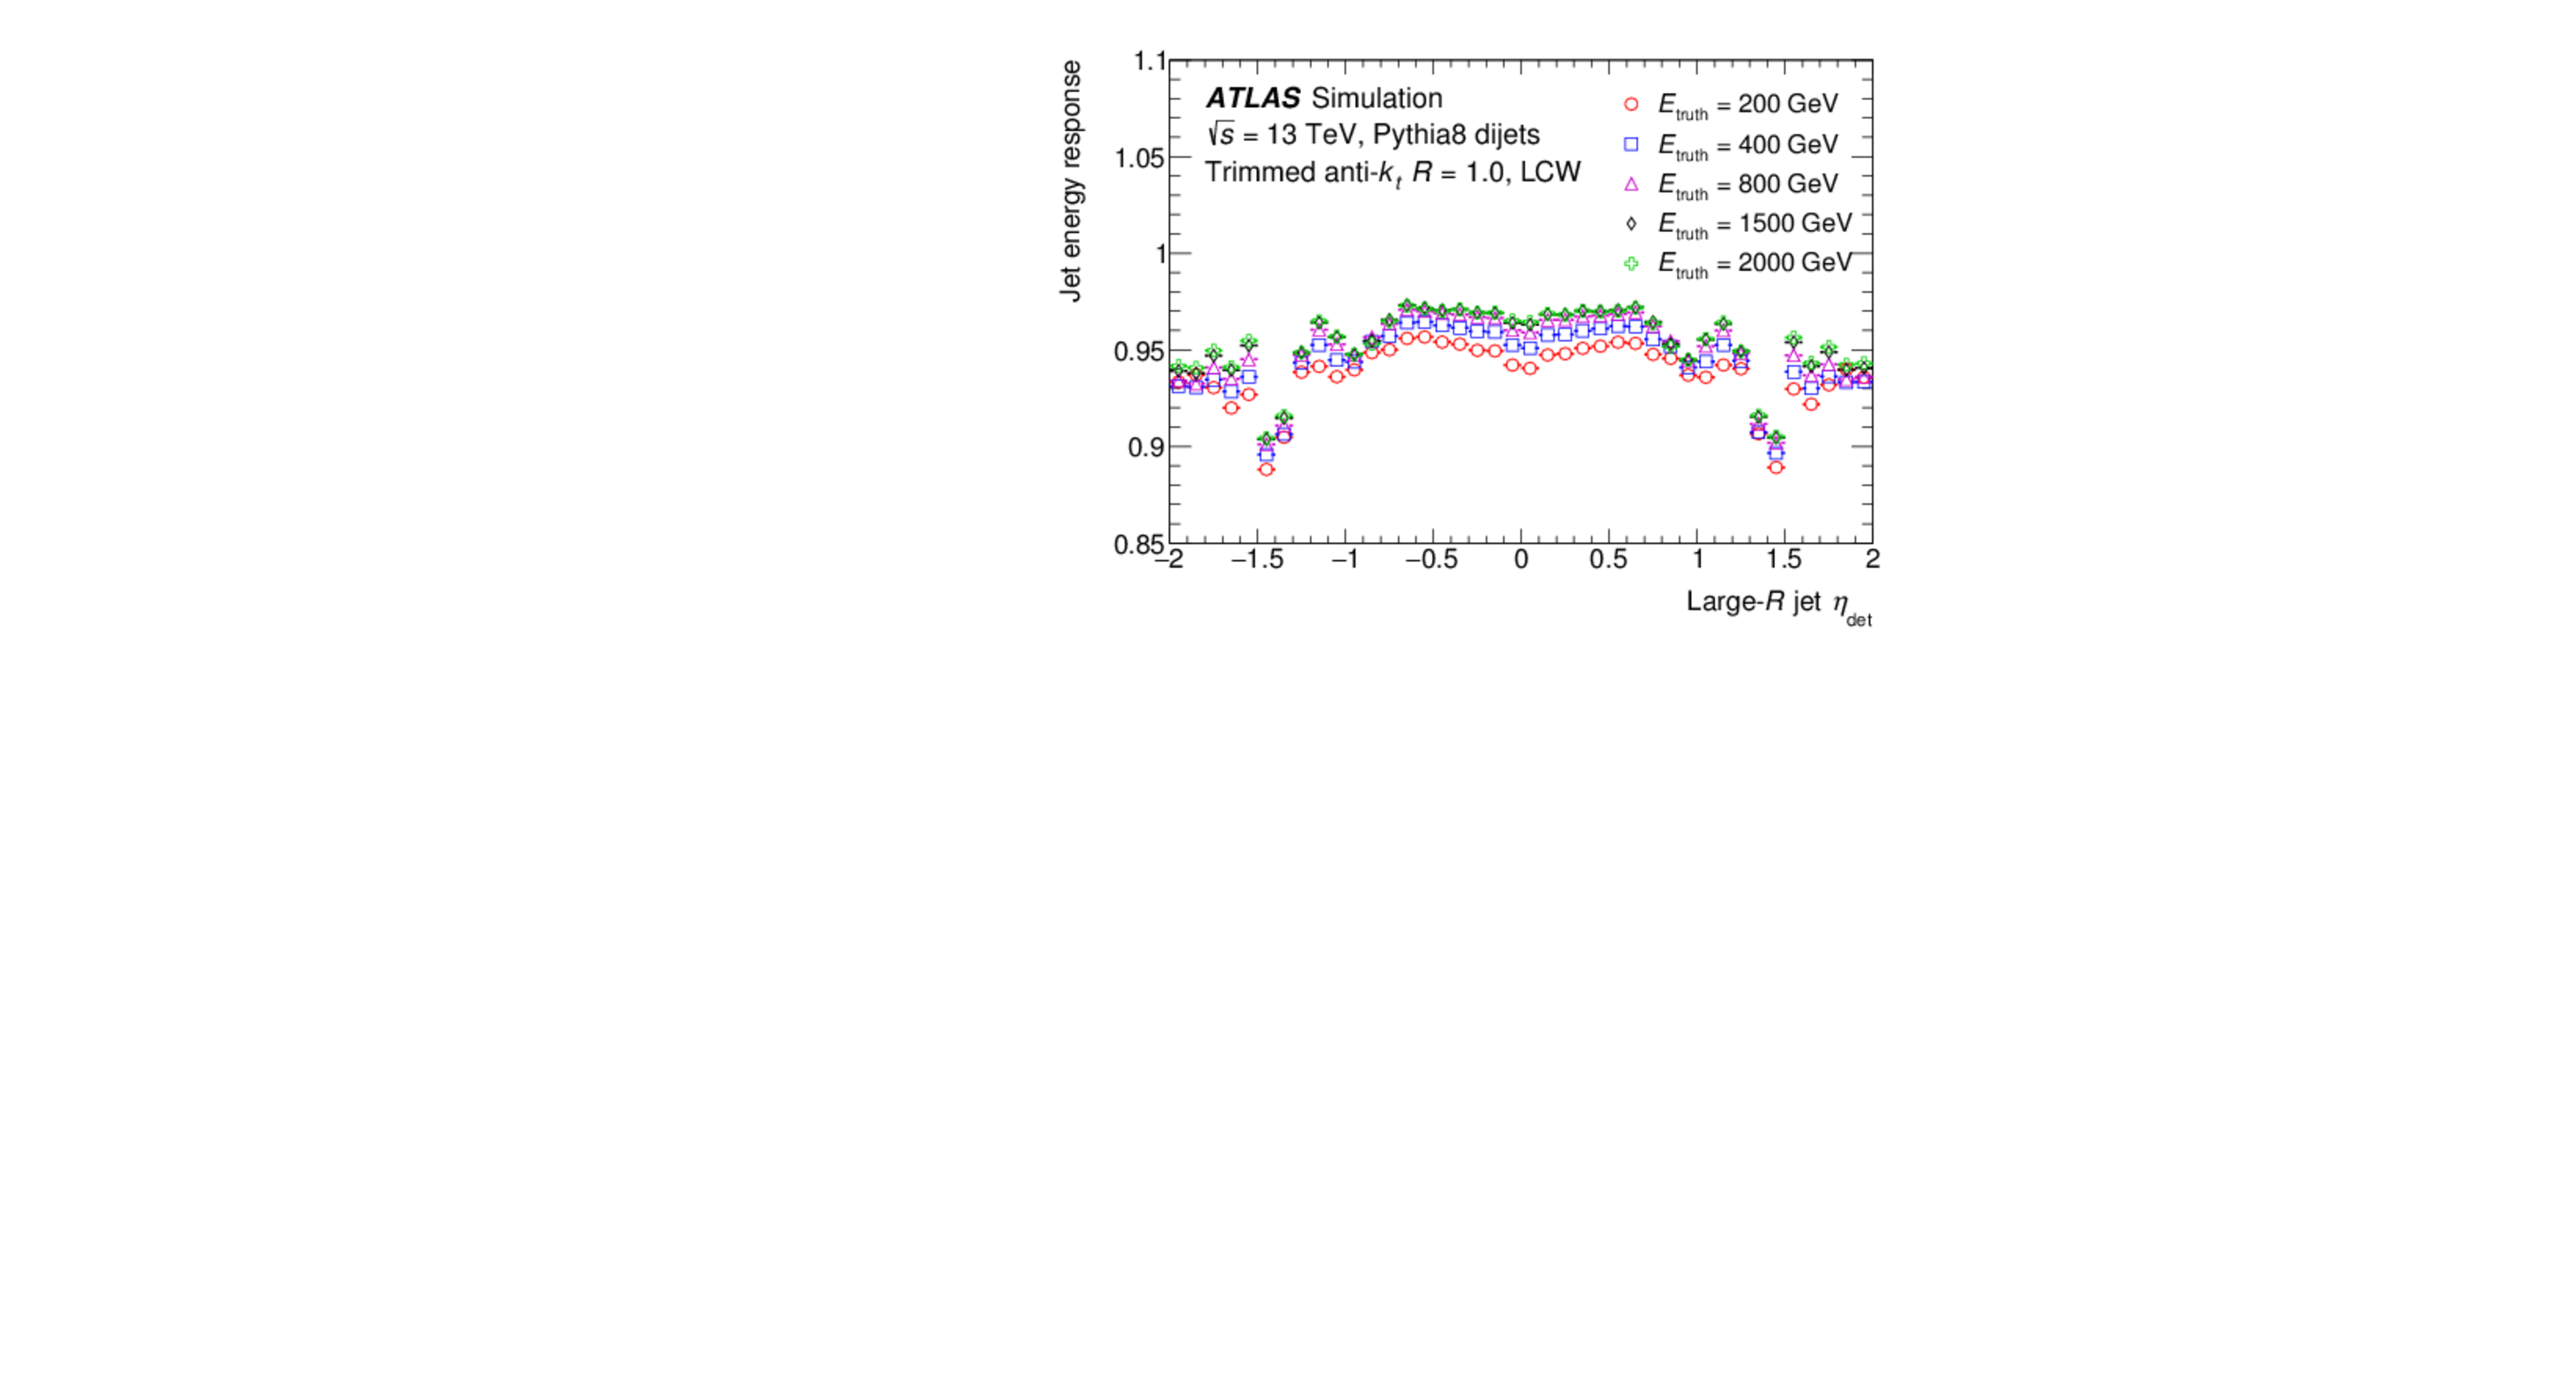
\includegraphics[width=0.45\textwidth,keepaspectratio]{figures/Reconstruction/responsept}
    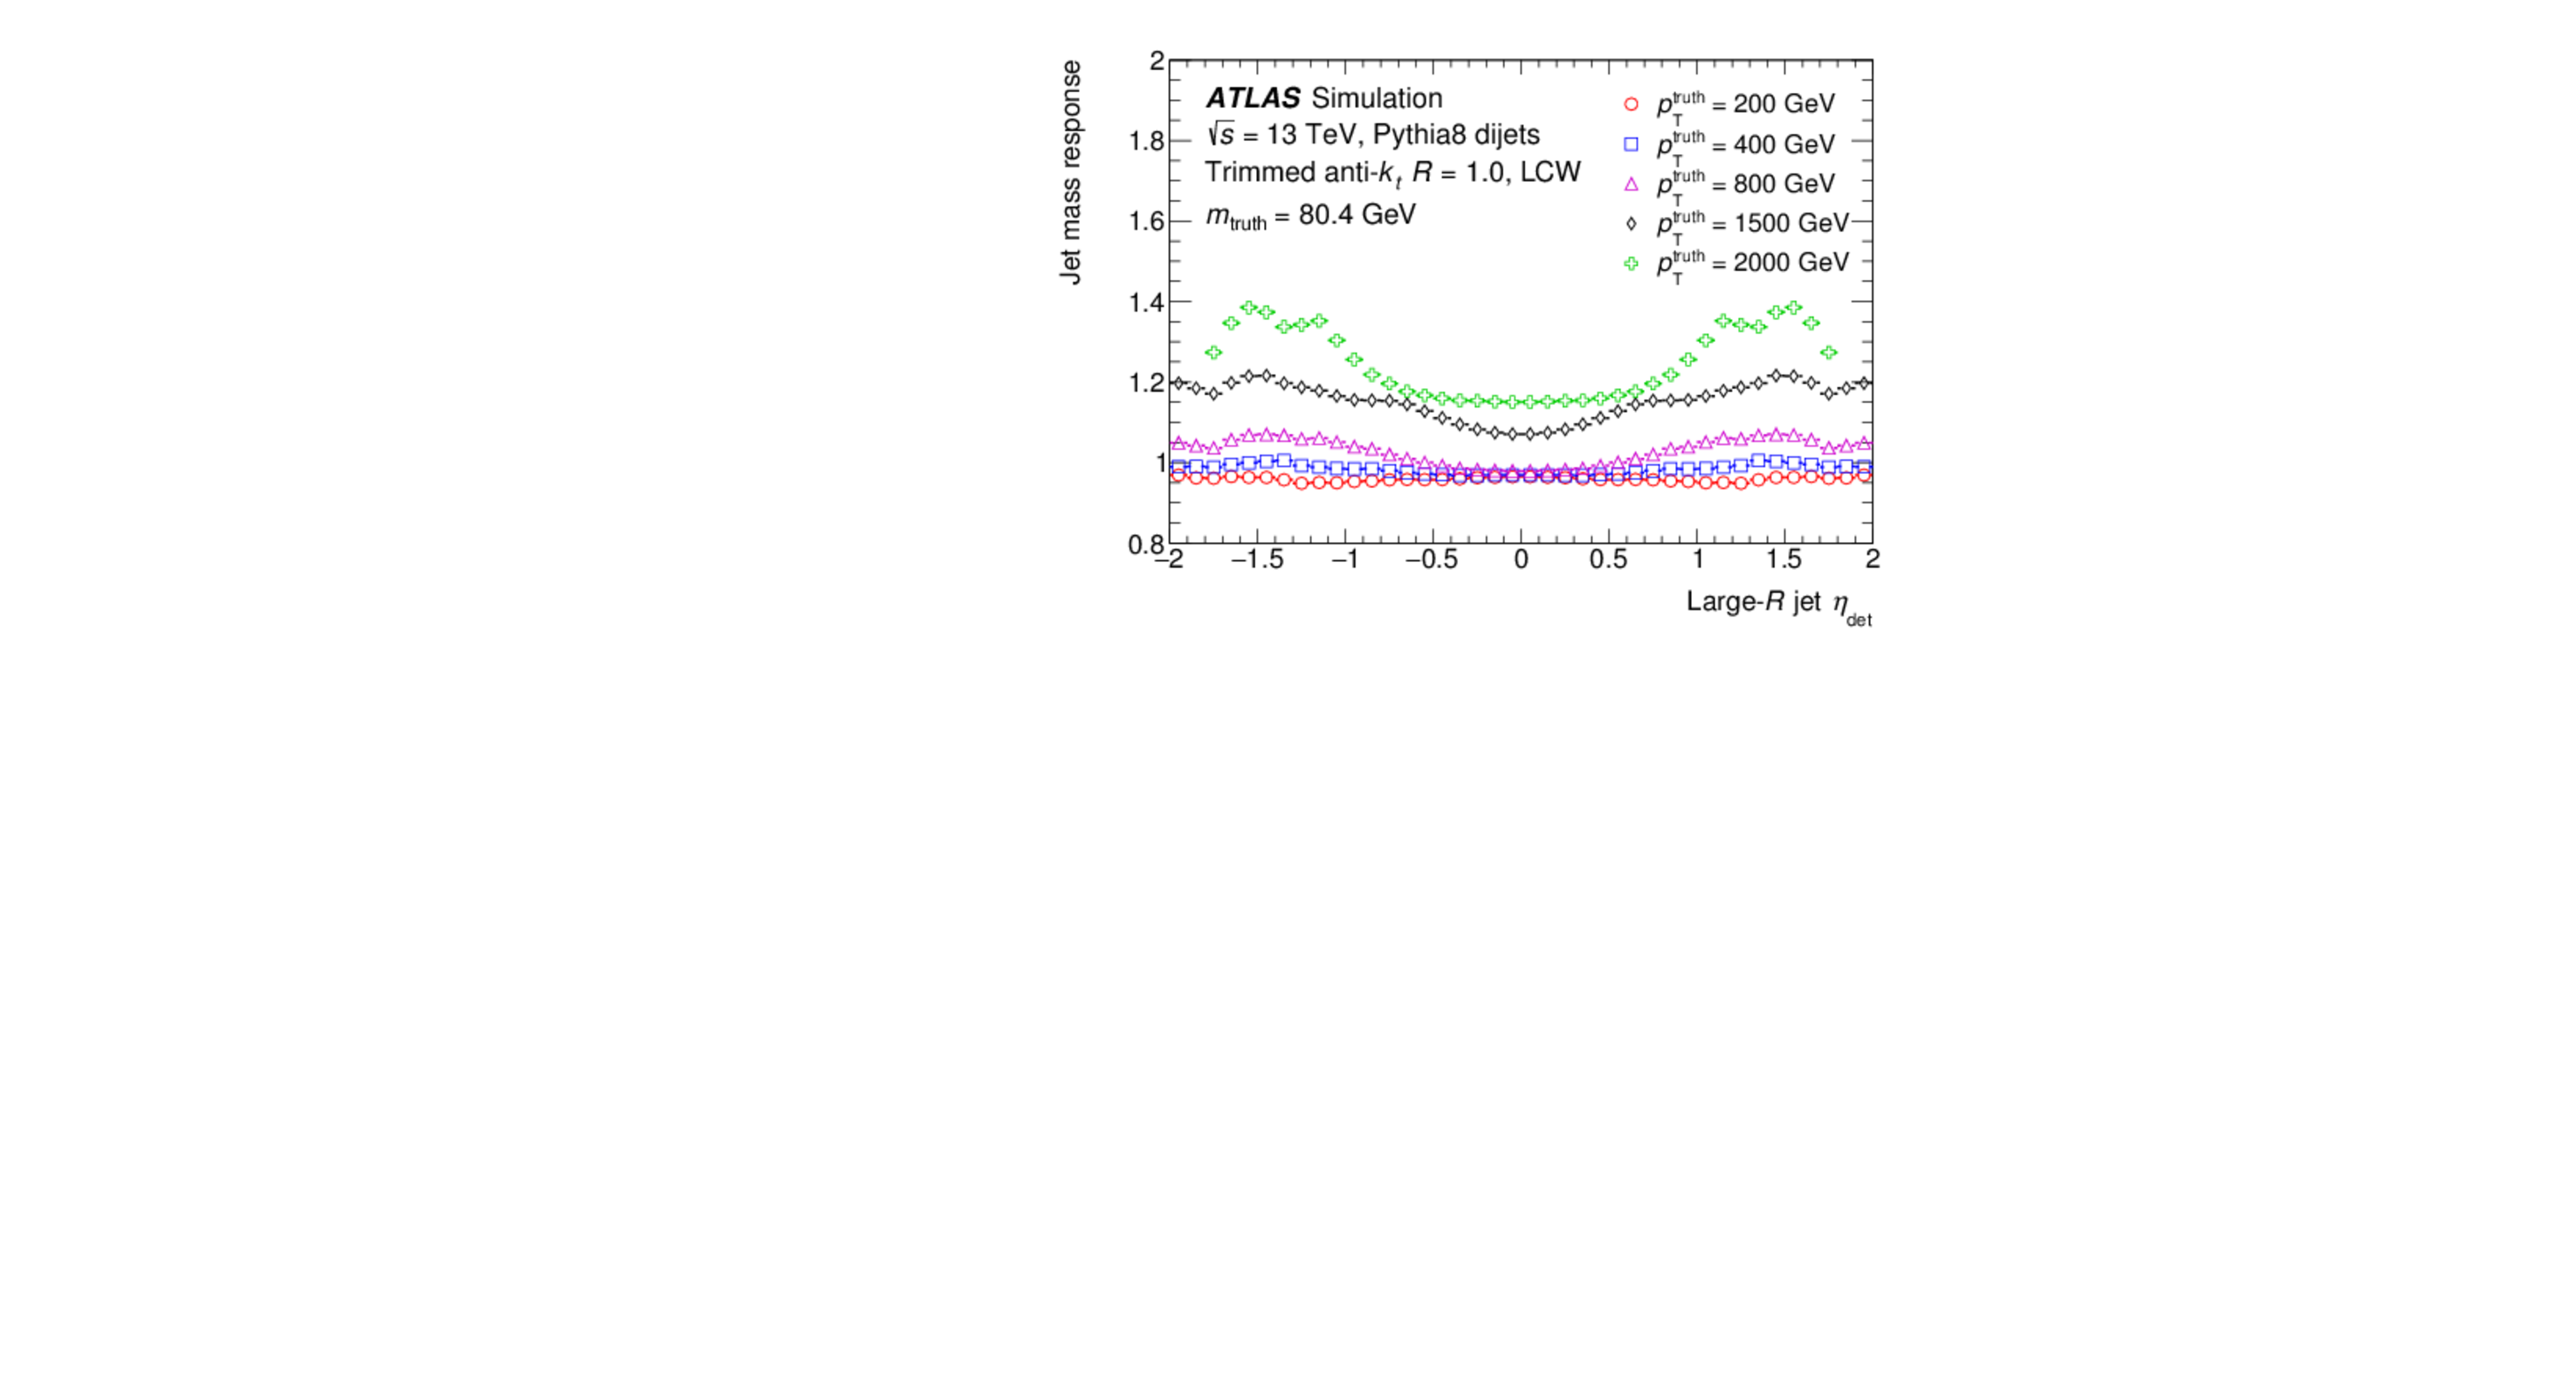
\includegraphics[width=0.45\textwidth,keepaspectratio]{figures/Reconstruction/responsemass}
    \caption{
    jet energy response of large-R jets \cite{JETM-2018-02}
    }
    \label{fig:largeRresponse}
    \end{center}
    \end{figure} 
    \item  \textbf{\sf{In-situ jet energy scale (JES) and jet mass scale (JMS) calibration}} \\
    In-situ calibration is applied for the remaining difference in the jet energy between the data and MC. 
    It is performed with a similar procedure with small-R jets. 
    The JES is calibrated in events where the jet recoils against a reference object, which are calibrated photon, reconstructed Z boson, or a system of well-measured small-R jets. The in-situ JMS calibration is performed after the application of the in-situ JES corrections. The jet mass response is measured from fits to the jet mass peaks formed from by high $p_\mathrm{T}$ W bosons and top quark decaying hadronically. 
    It is done by the $R_{trk}$ method using the independent measurements by the calorimeter and the inner tracker~\cite{JETM-2018-02}. 
\end{itemize}

\subsection{Jet substructure}
The large-R jet from boson has 2-prong structure, since it was originally collimated two quarks. This substructure can be the key to distinguish the boson jets to quark or gluon jets, which have 1-prong structure.
Figure~\ref{fig:jetsub} shows the schematic view of the substructure.
 \begin{figure}[tbp]
    \begin{center}
    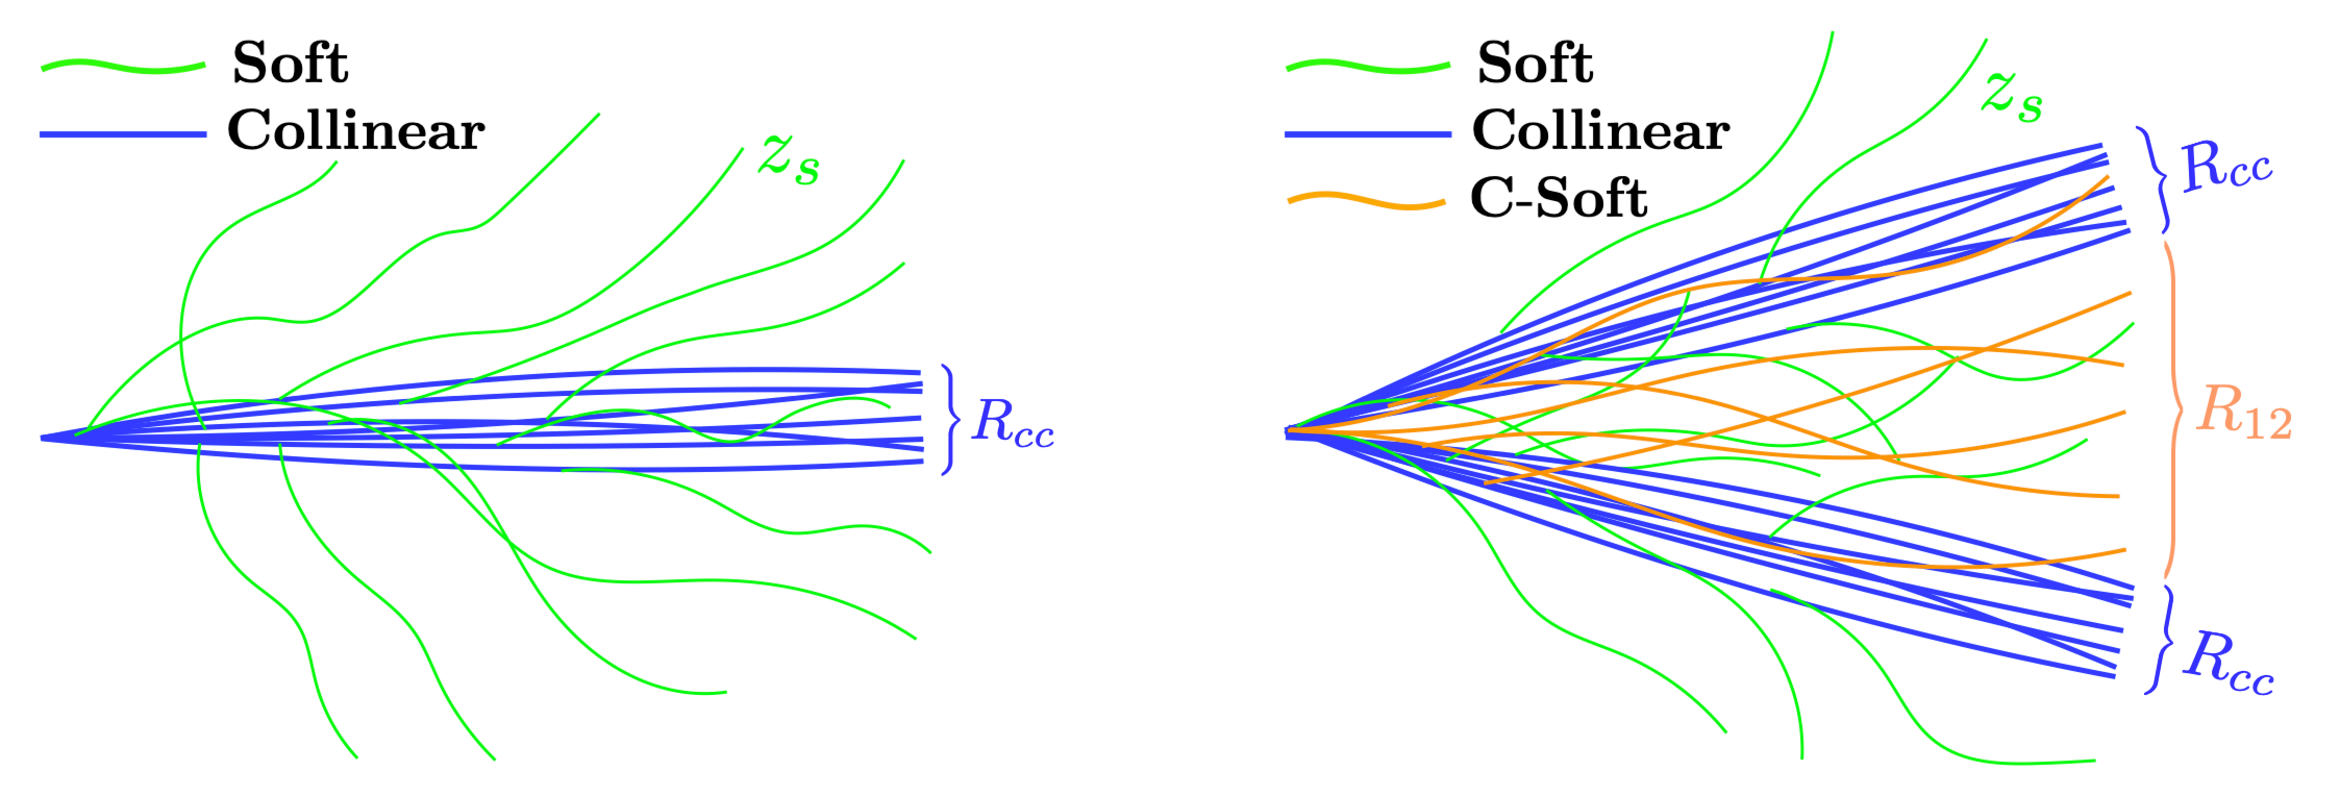
\includegraphics[width=0.80\textwidth,keepaspectratio]{figures/Reconstruction/jetsub}
    \caption{
    jet substructure \cite{Larkoski_2014}
    }
    \label{fig:jetsub}
    \end{center}
    \end{figure}
The jet substructure variable, $D_2$ is used to characterize the structure.  $D_2$ is defined as:
\begin{equation}
D_{2}^{(\beta)}=\frac{e_{3}^{(\beta)}}{\left(e_{2}^{(\beta)}\right)^{3}}
\end{equation}
where the 2 and 3-point energy correlation function $e_{n}^{(\beta)}$ is defined as:
\begin{equation}
\begin{aligned}
e_{2}^{(\beta)} &=\frac{1}{p_{T J}^{2}} \sum_{1 \leq i<j \leq n_{J}} p_{T i} p_{T j} R_{i j}^{\beta} \\
e_{3}^{(\beta)} &=\frac{1}{p_{T J}^{3}} \sum_{1 \leq i<j<k \leq n_{J}} p_{T i} p_{T j} p_{T k} R_{i j}^{\beta} R_{i k}^{\beta} R_{j k}^{\beta}
\end{aligned}
\end{equation}
where $p_{T J}$ is the transverse momentum of the jet with respect to the beam, $p_{T i}$ is the transverse momentum of particle $i$, and $n_{J}$ is the number of particles in the jet. 
The boost-invariant angle $R_{ij}^{2}=\left(\phi_{i}-\phi_{j}\right)^{2}+\left(y_{i}-y_{j}\right)^{2}$ is the distance in the azimuthrapidity plane and for infrared and collinear (IRC) safety, the angular exponent $\beta>0$. 
These energy correlation depends on how the soft and the collinear jet contributions are. The 1-prong and the 2-prong jets can be distinguished at the boundary of $e_{3}^{\beta=1} \sim\left(e_{2}^{\beta=1}\right)^{3}$ as shown in Figure~\ref{fig:phasespace23} \cite{Larkoski_2014}. 
\begin{figure}[tbp]
    \begin{center}
    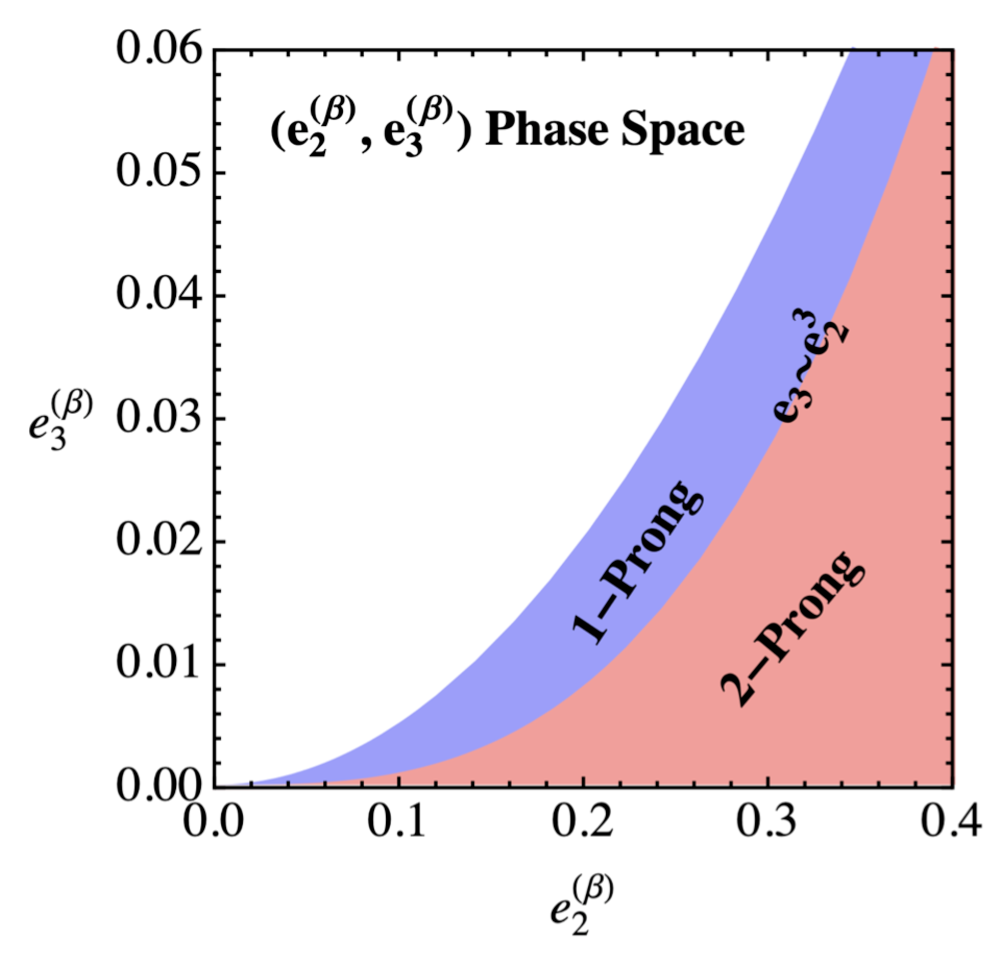
\includegraphics[width=0.45\textwidth,keepaspectratio]{figures/Reconstruction/phasespace23}
    \caption{
    boundaries of energy correlation function \cite{Larkoski_2014}
    }
    \label{fig:phasespace23}
    \end{center}
\end{figure}
The $D_2$ variable tends to get the lower value for 2-prong jet, boson jet while it tends to get the higher value for 1-prong jet, which is q/g jet.
\subsection{Boosted Boson Tagger}
The 3-variable cut-based tagger, that relies on $D_2$, jet mass, and the number of the tracks is used for identifying the large-R jet from W/Z boson and to reject the other SM background processes~\cite{ATL-PHYS-PUB-2020-017} . 
The combined mass, reconstructed as the weighted sum of masses from calorimeter information and from mixed calorimeter and tracking information, is exploit since the W/Z decaying jet mass peaks around 80/91~GeV. 
The 2-prong energy structure inside jet which is characterized by $D_2$ is used.
The number of track has been found to improve background rejection for a fixed signal efficiency~\cite{EXOT-2013-08} due to the rejection of jets seeded by gluons.  
Unlike jets from massive boson decays in which the hadron multiplicity is essentially independent of the jet $p_\mathrm{T}$, energetic gluon jets are typically composed of more hadrons, so the number of charged-particle tracks associated with the original, ungroomed jet is required to be small. 
The tagger provides two fixed working points defined at 50\% and 80 \% signal efficiency. 
Figure~\ref{fig:bosonTagger} shows the measured signal efficiency plot of the boson tagger and the measured background rejection plot for 50~\% efficiency working point.
\begin{figure}[tbp]
    \begin{center}
    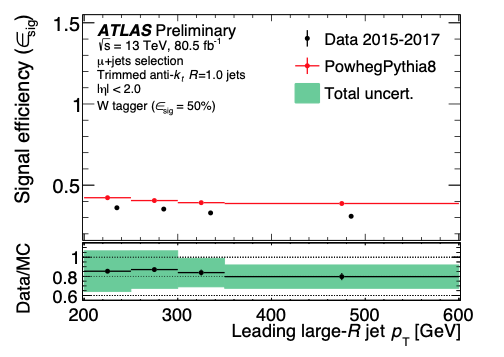
\includegraphics[width=0.47\textwidth,keepaspectratio]{figures/Reconstruction/bosontaggersignaleff}
    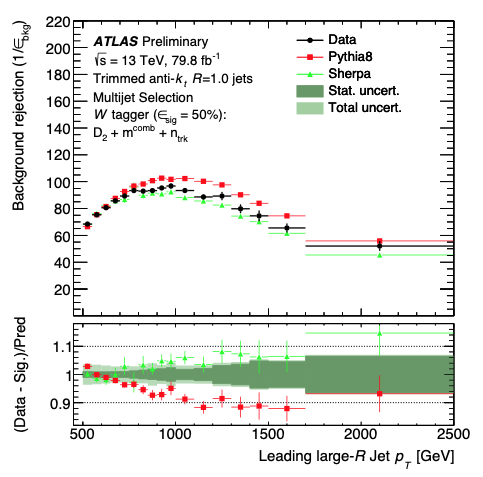
\includegraphics[width=0.42\textwidth,keepaspectratio]{figures/Reconstruction/bosontaggerrejection}
    \caption{
     Measured signal efficiency (left) and background rejection (right) for 50~\% W tagger \cite{ATL-PHYS-PUB-2020-017}
    }
    \label{fig:bosonTagger}
    \end{center}
\end{figure}

%large-R jets are required to be $p_T$ > 200~GeV and $|\eta| <2.0$, and jet mass > 50~GeV.
\section{Missing Transverse Momentum}
The particle such as neutrinos traverses the whole detector and cannot be detected in the detector, as the Figure~\ref{fig:ParticlePath} shows. 
Those invisible particles are reconstructed by using the imbalance of the transverse momenta. 
It is calculated by the following formula:
\begin{equation}
\mathbf{E}_{\mathbf{T}}^{\text {miss }}=-\sum_{i \in\{\text { hard objects }\}} \mathbf{p}_{\mathbf{T}, \mathbf{i}}-\sum_{j \in\{\text { soft objects }\}} \mathbf{p_{T,\mathbf{j}}}
\end{equation}
by taking the negative sum of the momenta of detected objects, electrons, muons, and jets and additionally, so called soft terms, which are charged-particle tracks not matched to the reconstructed objects~\cite{PERF-2016-07}.
